\documentclass[9pt]{beamer}
\usepackage[utf8]{inputenc}
\usepackage[T1]{fontenc}
%\usepackage{verdana} %?
\usepackage[russian]{babel}
\usepackage{graphicx}
\usepackage{tikz}
\usepackage{pifont}
\usetheme{Warsaw}
\usecolortheme{orchid}
\setbeamertemplate{frametitle}
{
    \begin{beamercolorbox}[sep=0.3cm,ht=2.2em,wd=\paperwidth]{frametitle}
        \vbox{}\vskip-2.0ex%
        \strut\insertframetitle\strut
        \vskip-0.8ex%
    \end{beamercolorbox}
}

%\renewcommand{\familydefault}{verdana}
\setbeamerfont{block title}{size=\normalsize}
\title[World development indicators]{\huge World development indicators}
\subtitle[Which country will develop more]{\large Which country will develop more}
\author[Moawad, Comandini, Isaeva, Schiavon, Snesarevskii] {{\Large Group 12:\\}Stefano Moawad\\Leonardo Comandini\\Diana Isaeva\\Andrea Schiavon\\Viktor Snesarevskii}
\date{April-May 2017}
\usebackgroundtemplate{\tikz\node[opacity=0.3] {\vbox to \paperheight{\vfil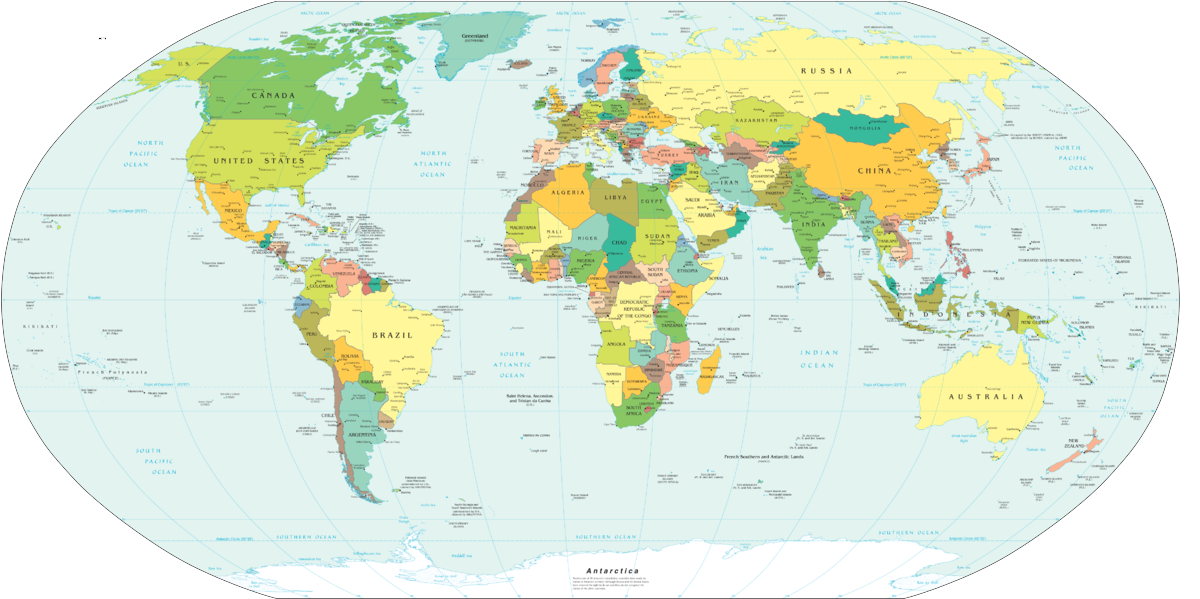
\includegraphics[width=\paperwidth]{map}\vfil}};}

\begin{document}
	\begin{frame}
	\titlepage
	\vfill
	\begin{flushright}
		
\includegraphics[height=.7cm]{kaggle.png}\quad
		
\includegraphics[height=.7cm]{worldbank.jpg}
	\end{flushright}
\end{frame}

\begin{frame}{Our Goals} 
Abstract: “… individuate the best countries where to invest, w.r.t. different economical and social fields"
\begin{itemize}  % elements appears one by one
	\only<1-1>{\item Best = ?}
	\only<2->{\item Best = upcoming largest development}
	\only<3->{\item Development = ?}
	\only<4->{\item Invest = ?}
\end{itemize}
\end{frame}

% snapshot raw dataset
\begin{frame}{Raw dataset}
\begin{block}{Indicators (5 656 458 x 6)}
\scriptsize
\begin{tabular}{*{6}{l}}
	Country name &
	\only<1-1>{Country code}\only<2->{\!\!\tikz[baseline]\node[anchor=base,draw=red]{Country code};}& 
	\!\! Indicator name & \!\! Indicator code & Year & 
	\only<1-1>{Value}\only<2->{\!\!\tikz[baseline]\node[anchor=base,draw=cyan]{Value};}
\end{tabular}
\end{block}
\begin{block}{Country (247 x 31)}
\scriptsize
\begin{tabular}{*{5}{l}}
	\only<1-1>{Country code}\only<2->{\!\!\tikz[baseline]\node[anchor=base,draw=red]{Country code};}& 
	Short name & Table name & Long name & Alpha 2 code \\[.15cm]
	Currency unit & Special notes &
	\only<1-1>{Region}\only<2->{\!\!\tikz[baseline]\node[anchor=base,draw=green]{Region};}&
	Indice group & \textbf{etc...}
\end{tabular}
\end{block}

\begin{block}{Country notes (4 857 x 3)}
\scriptsize
\begin{tabular}{*{5}{l}}
	\only<1-1>{Country code}\only<2->{\!\!\tikz[baseline]\node[anchor=base,draw=red]{Country code};}&
	\only<1-1>{Series code}\only<2->{\!\!\tikz[baseline]\node[anchor=base,draw=blue]{Series code};}&
	Description
\end{tabular}
\end{block}
\begin{block}{Series (1 345 x 20)}
\scriptsize
\begin{tabular}{*{4}{l}}
	\only<1-1>{Series code}\only<2->{\!\!\tikz[baseline]\node[anchor=base,draw=blue]{Series code};}&
	Topic & Indicator name\!\! & Short definition \\[.15cm] Long definition & 
	\only<1-1>{Unit of measure}\only<2->{\!\!\tikz[baseline]\node[anchor=base,draw=orange]{Unit of measure};}&
	Periodicity  & \textbf{etc...}
\end{tabular}
\end{block}
\begin{block}{Series notes (369 x 3)}
\scriptsize
\begin{tabular}{*{5}{l}}
	\only<1-1>{Series code}\only<2->{\!\!\tikz[baseline]\node[anchor=base,draw=blue]{Series code};}&
	\only<1-1>{Year}\only<2->{\!\!\tikz[baseline]\node[anchor=base,draw=black]{Year};}&
	Description
\end{tabular}
\end{block}
\end{frame}

\begin{frame}{Examples of indicators}
\centering
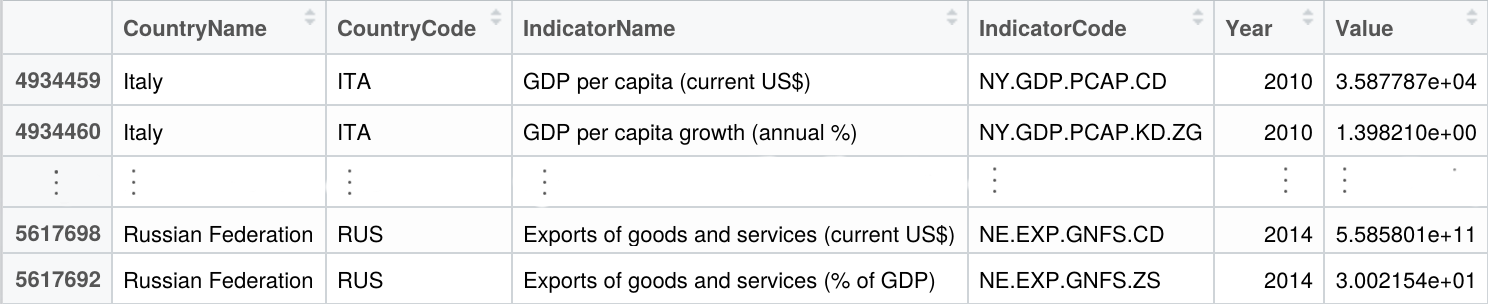
\includegraphics [width=\textwidth]{indicators.png}
\end{frame}


\usebackgroundtemplate{}
\begin{frame}
	\centering
	\includegraphics[width=\textwidth]{3Dmatrix.png}
\end{frame}
\usebackgroundtemplate{\tikz\node[opacity=0.3] {\vbox to \paperheight{\vfil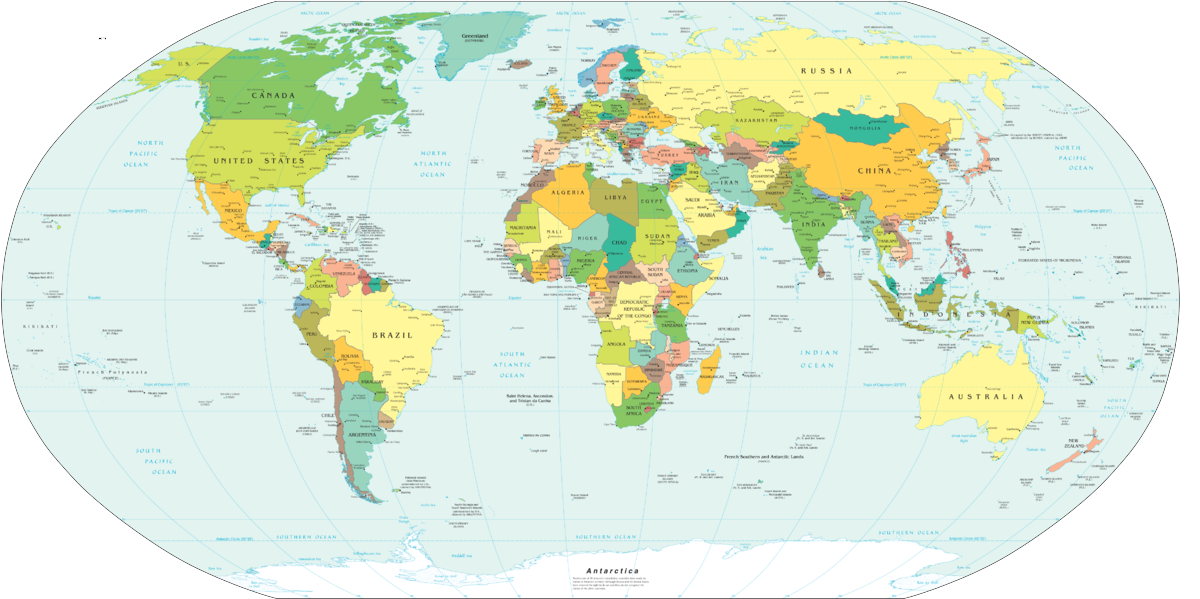
\includegraphics[width=\paperwidth]{map}\vfil}};}
%\begin{frame}
%\begin{figure}
%\centering
%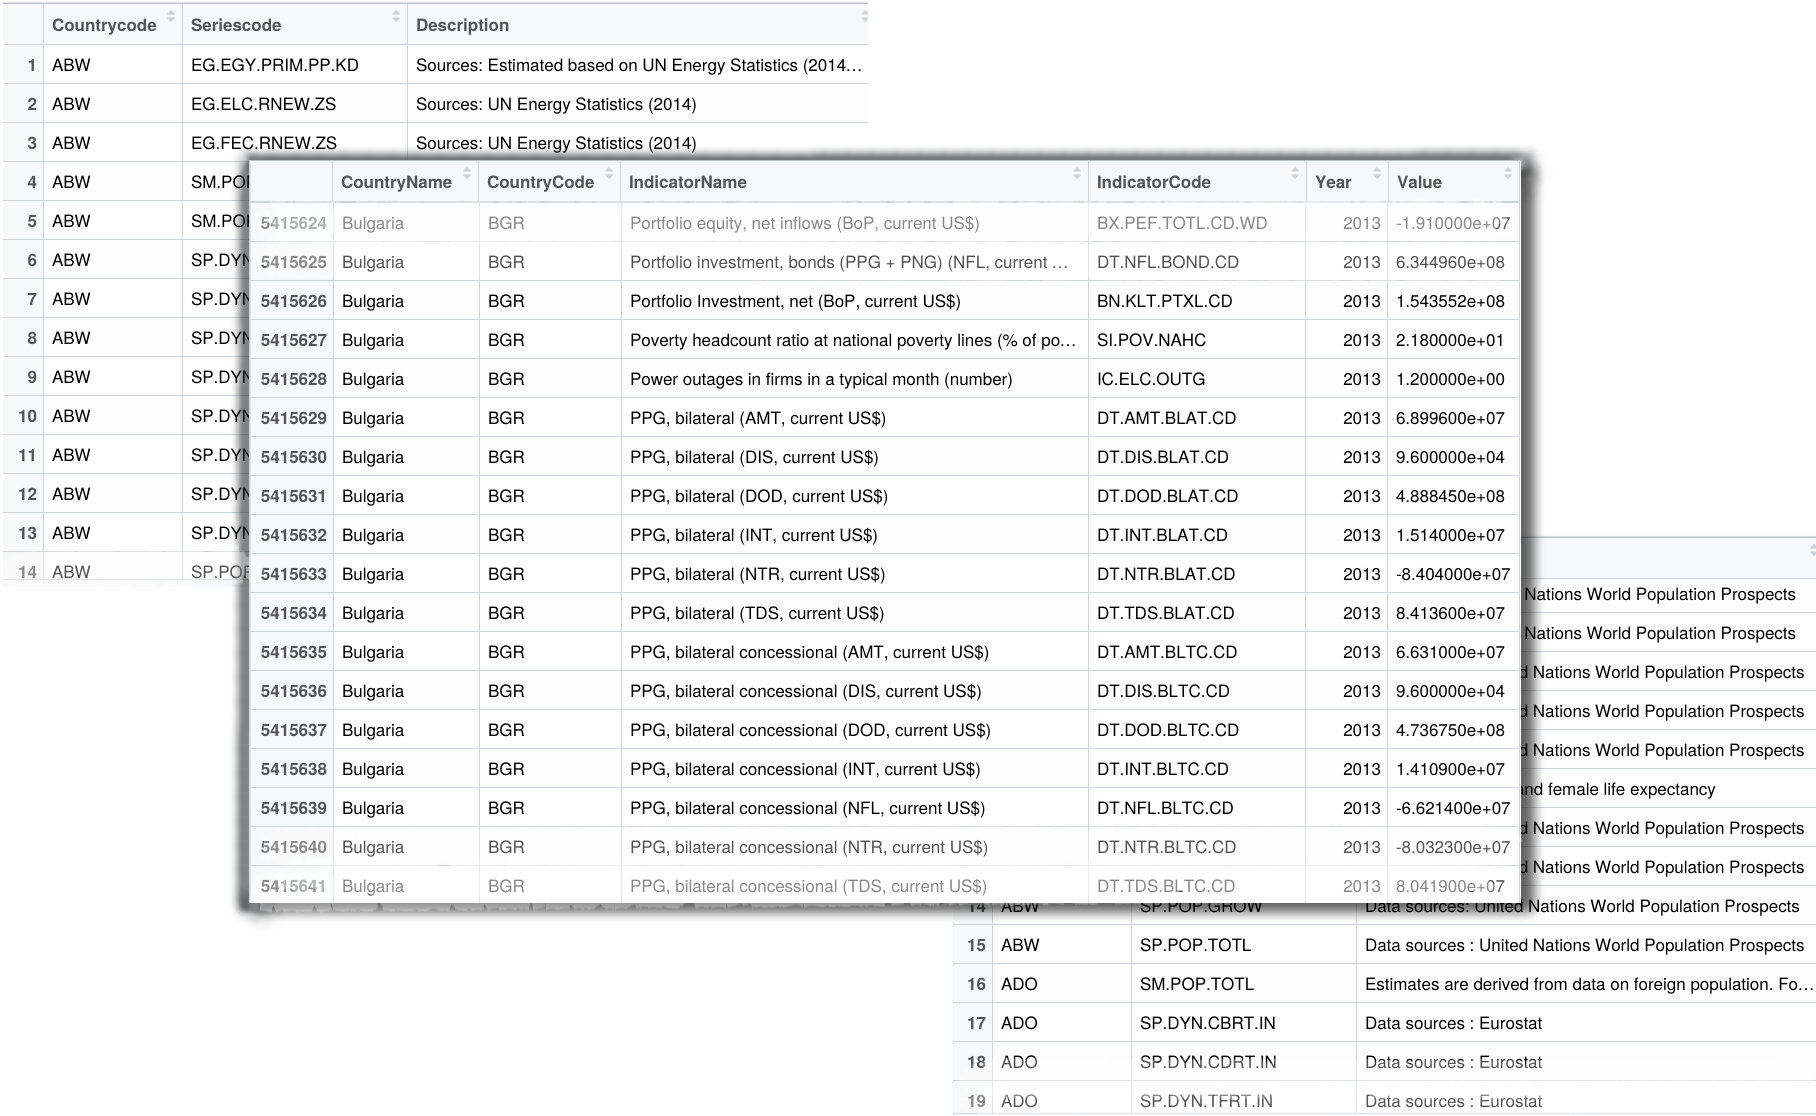
\includegraphics[width=\textwidth]{tables_2.png}
%\end{figure}
%\end{frame}

\begin{frame}
Looking at \textit{Indicators} as a 3D matrix leads to some problems
\begin{itemize} [<+->]
\item \textbf{Years} \ding{221} not homogeneous
\item \textbf{Countries} \ding{221} small ones
\item \textbf{Indicators} \ding{221} too varied to choose easily
\end{itemize}
\end{frame}

\begin{frame}
\begin{figure}
\centering
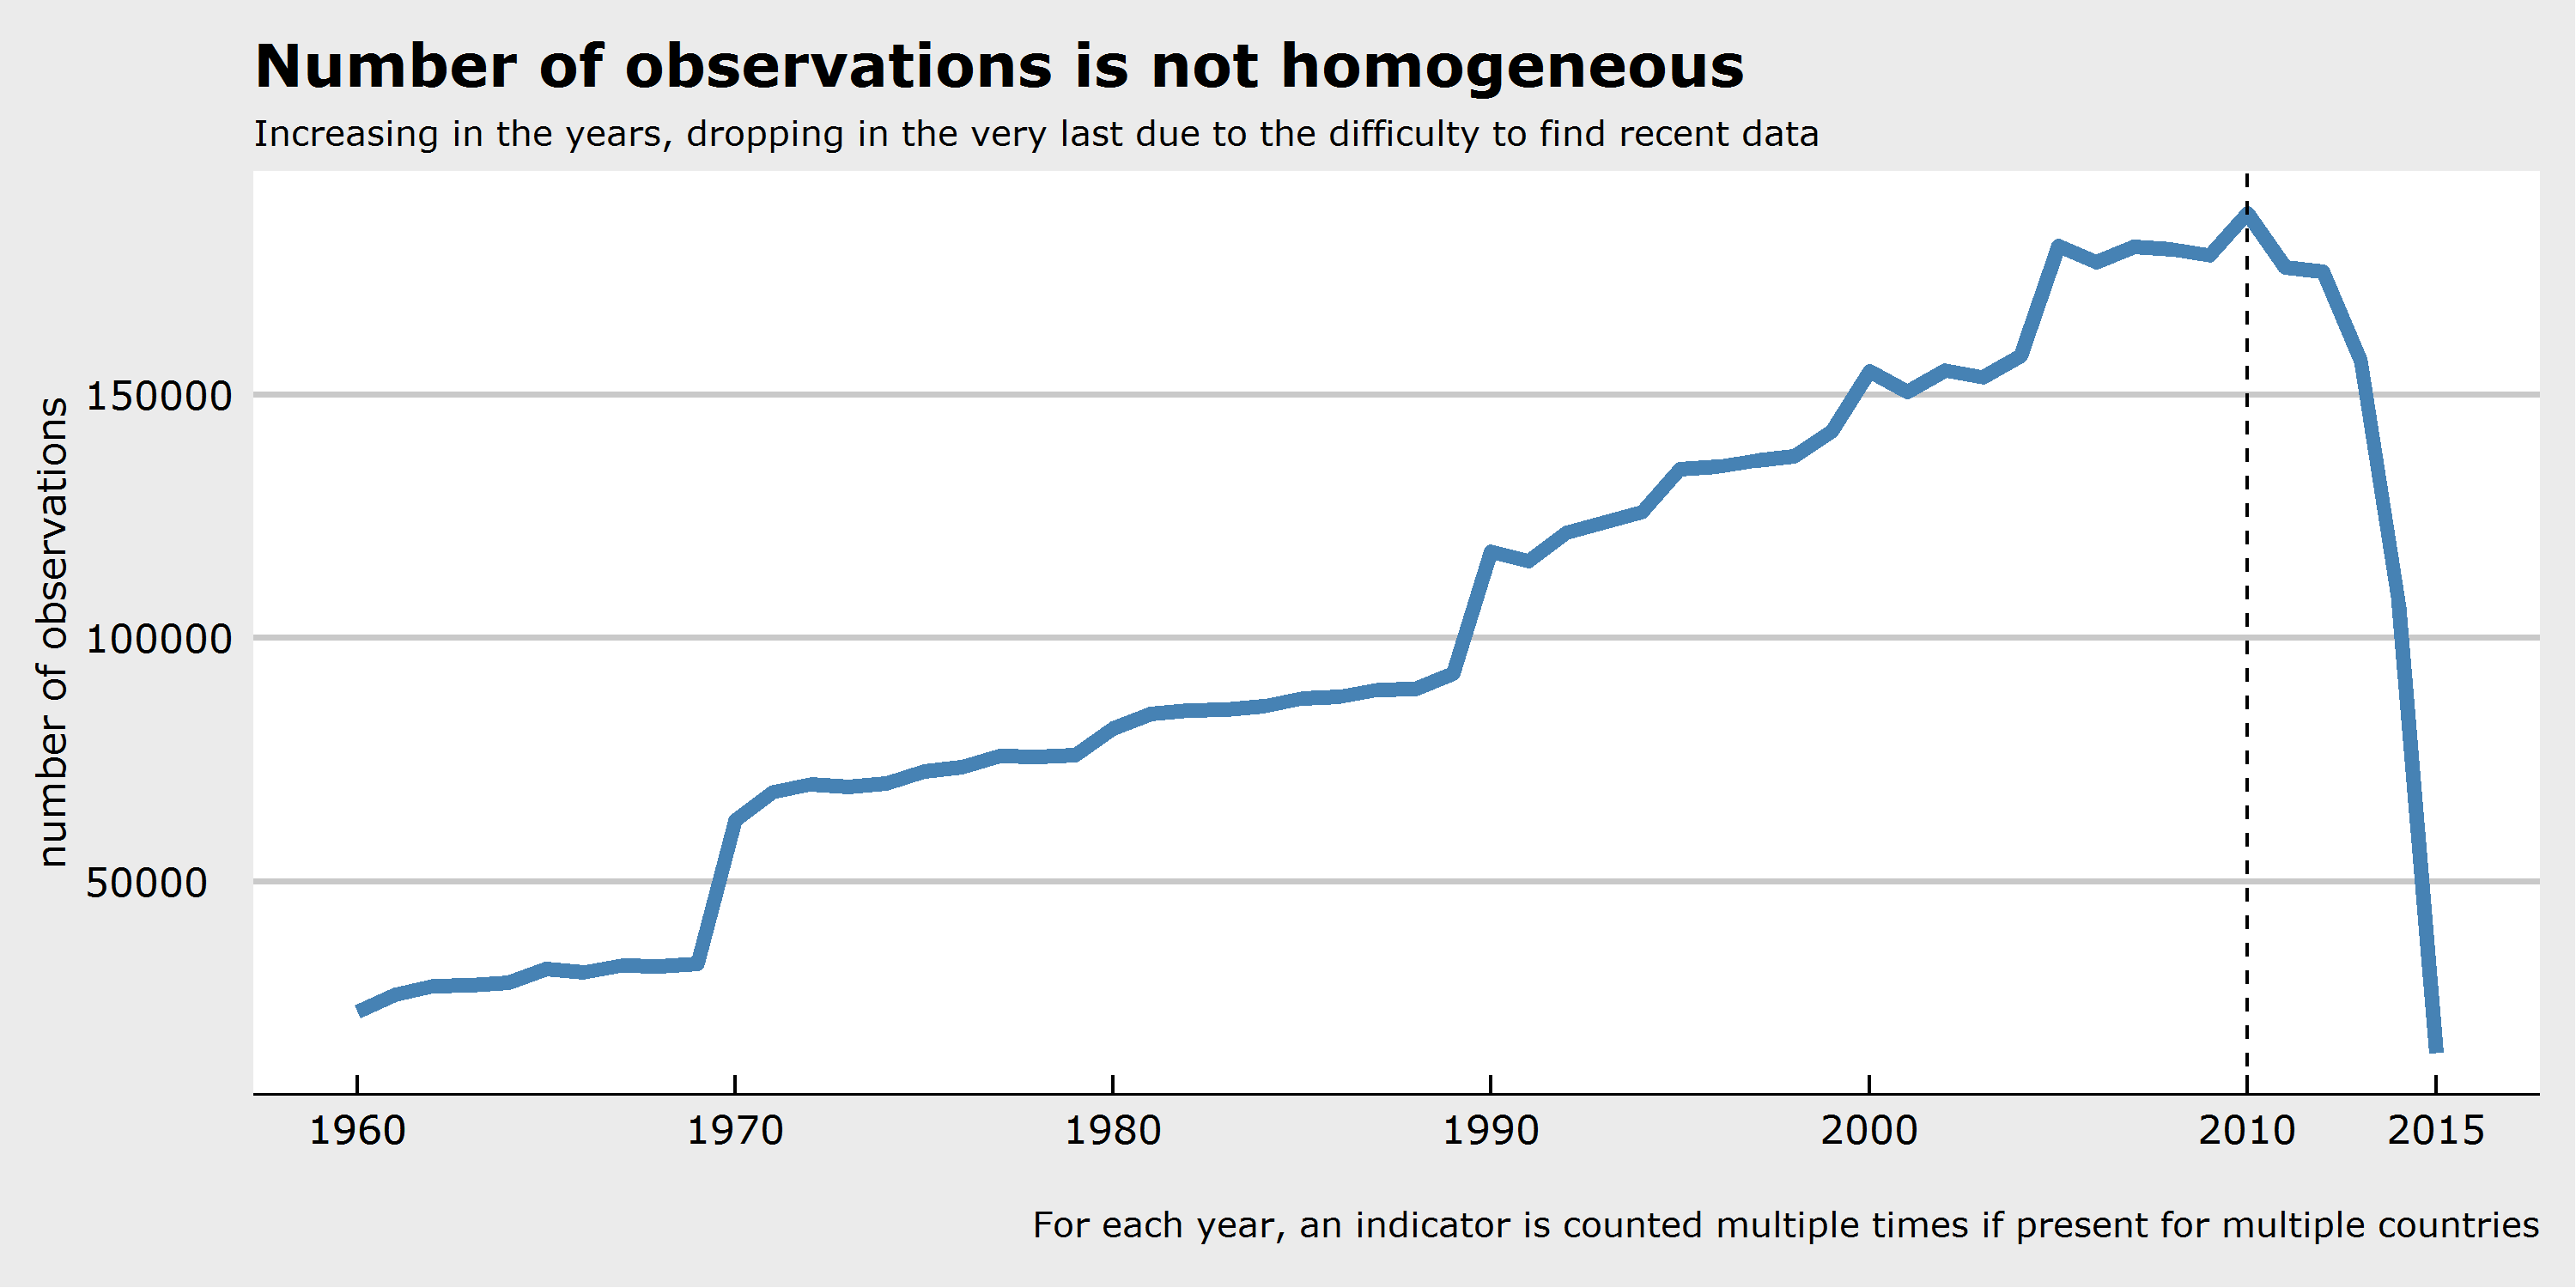
\includegraphics[width=\textwidth]{plot0001.png}
\end{figure}
\end{frame}

\begin{frame}
\begin{figure}
\centering
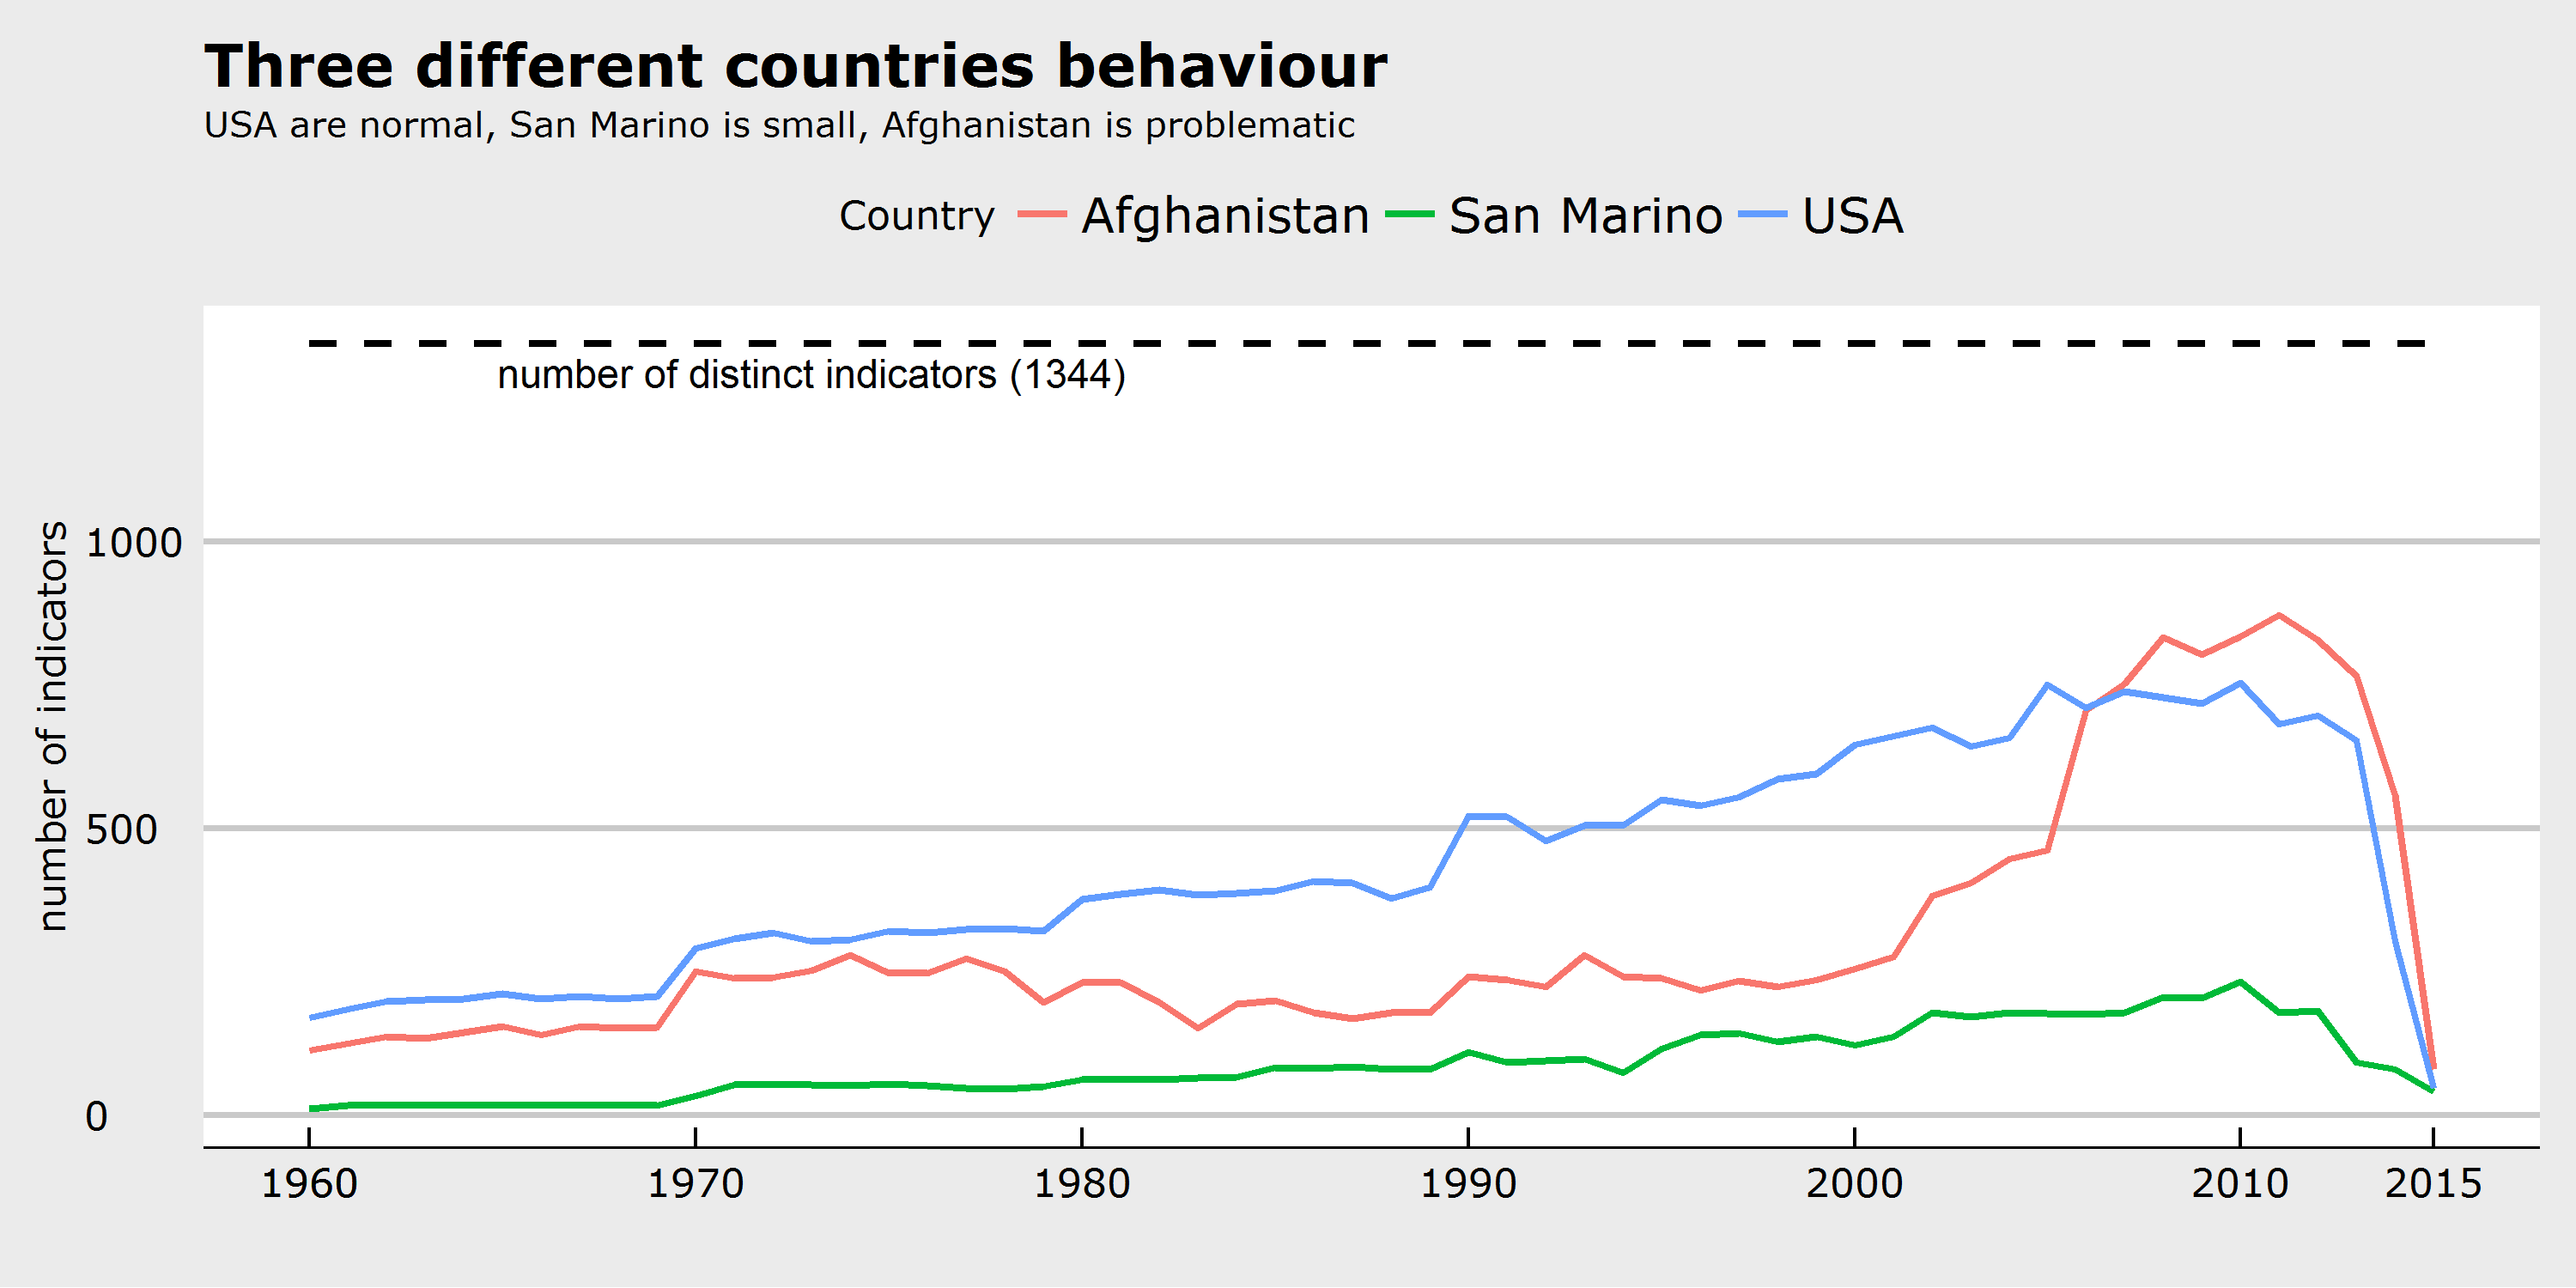
\includegraphics[width=\textwidth]{plot0002.png}
\end{figure}
\end{frame}

\begin{frame}
\begin{figure}
\centering
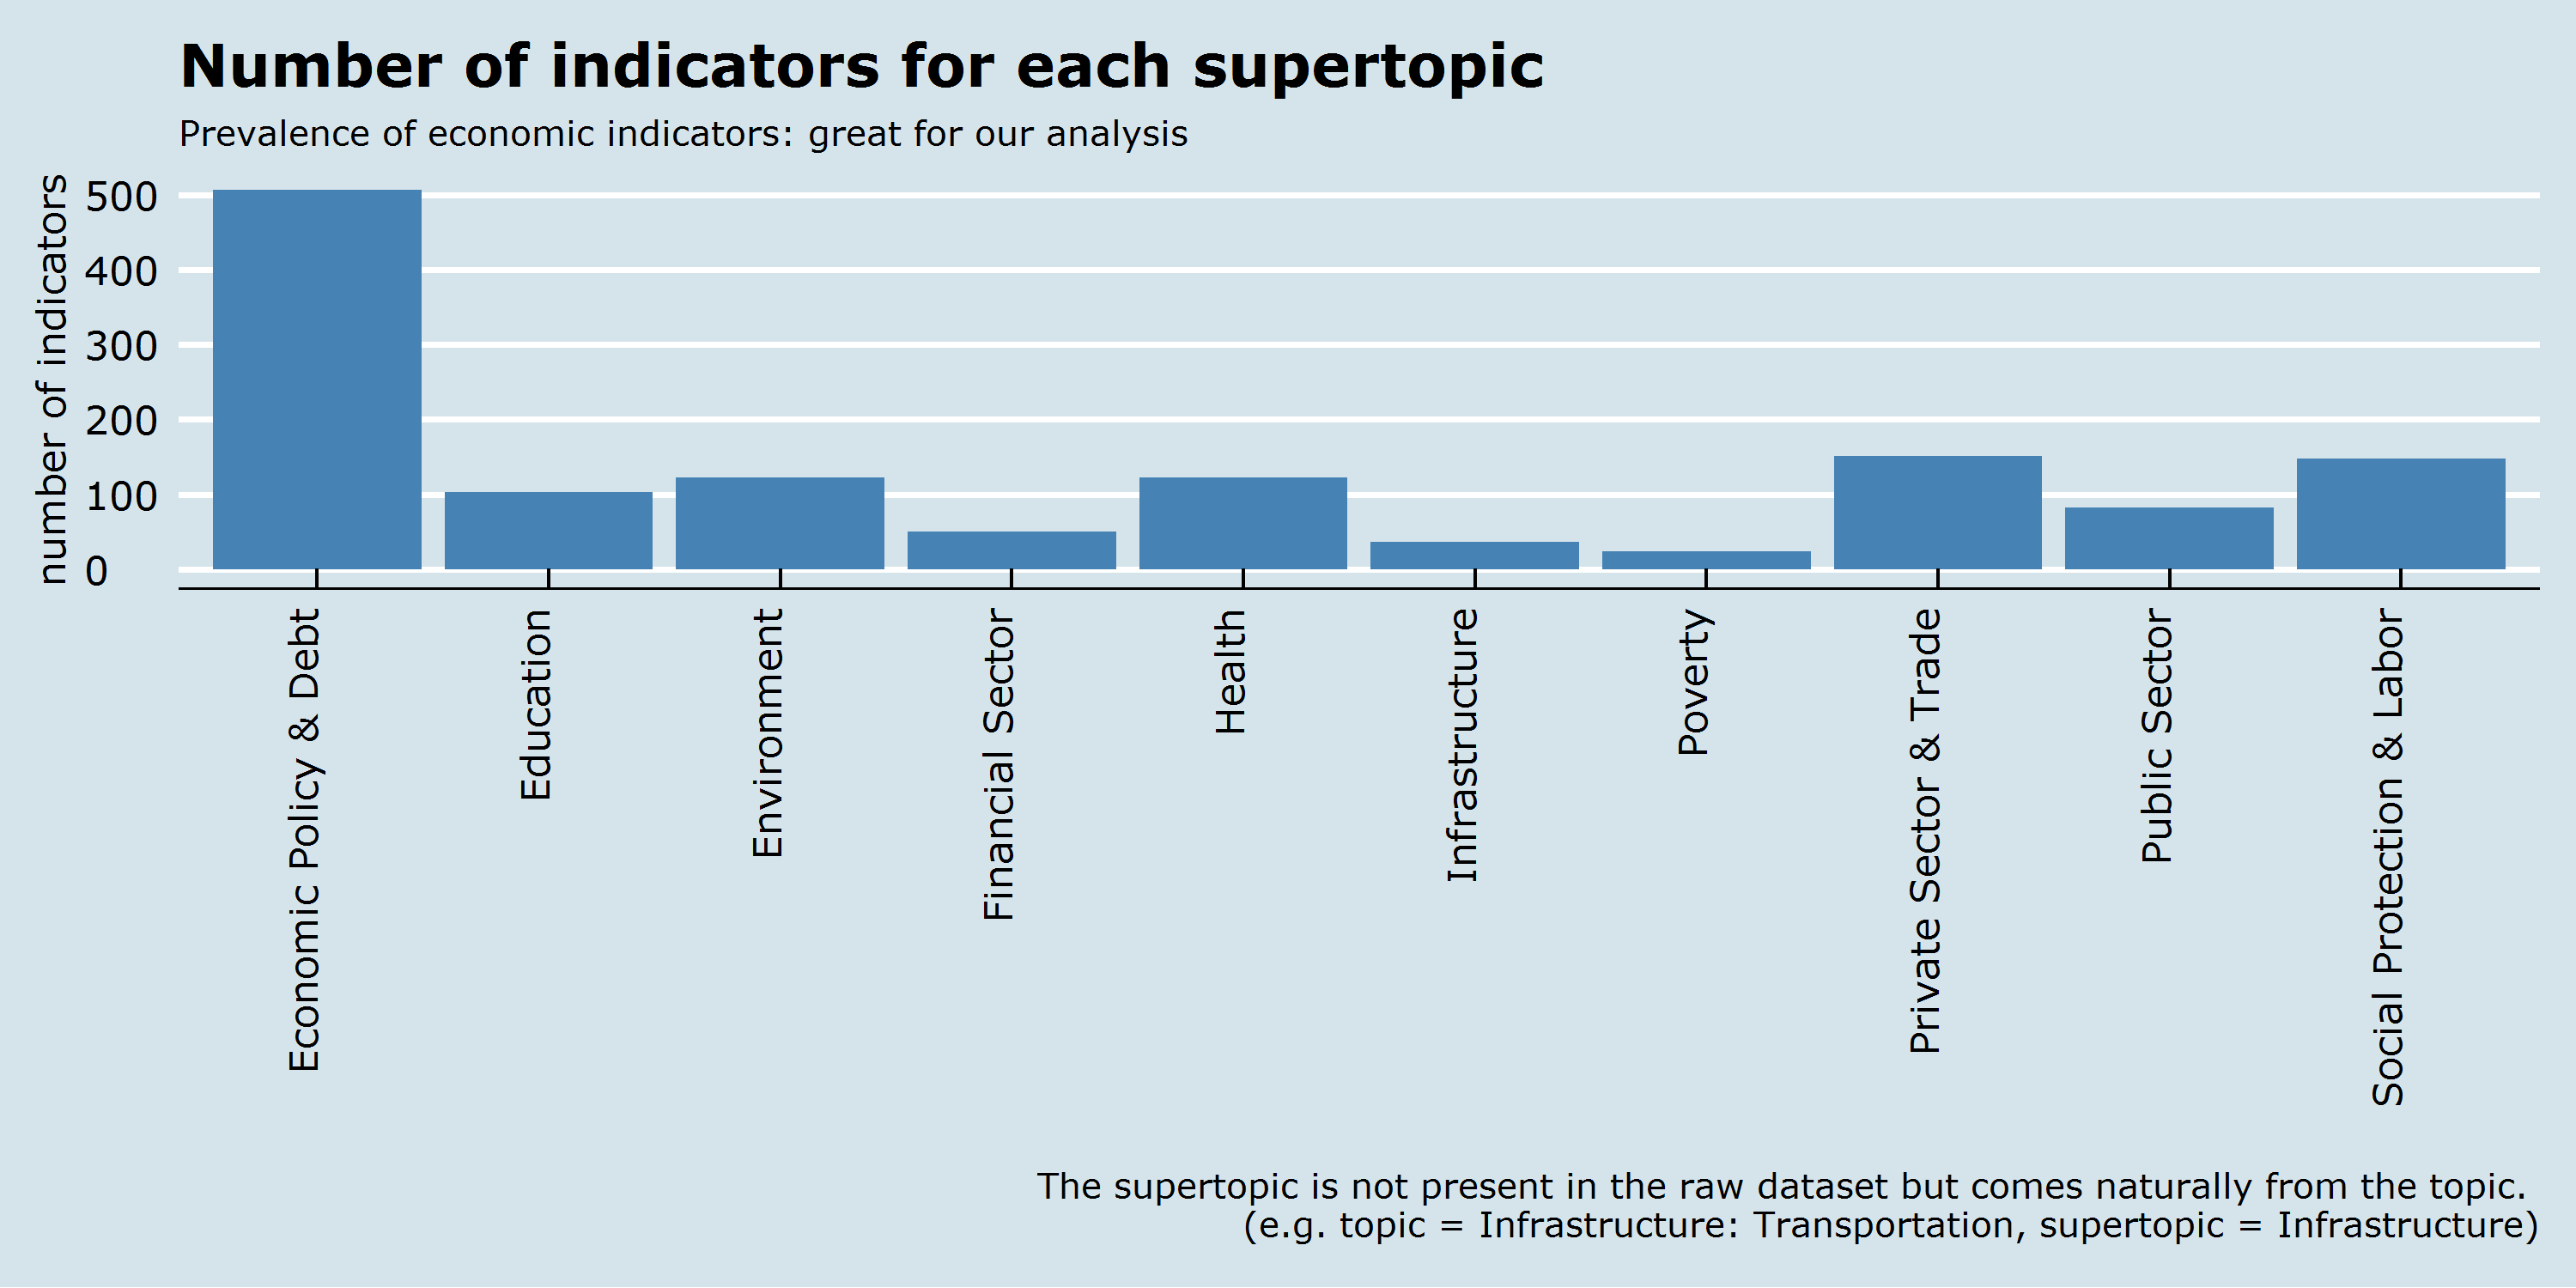
\includegraphics[width=\textwidth]{plot0003.png}
\end{figure}
\end{frame}

\begin{frame}
\begin{figure}
\centering
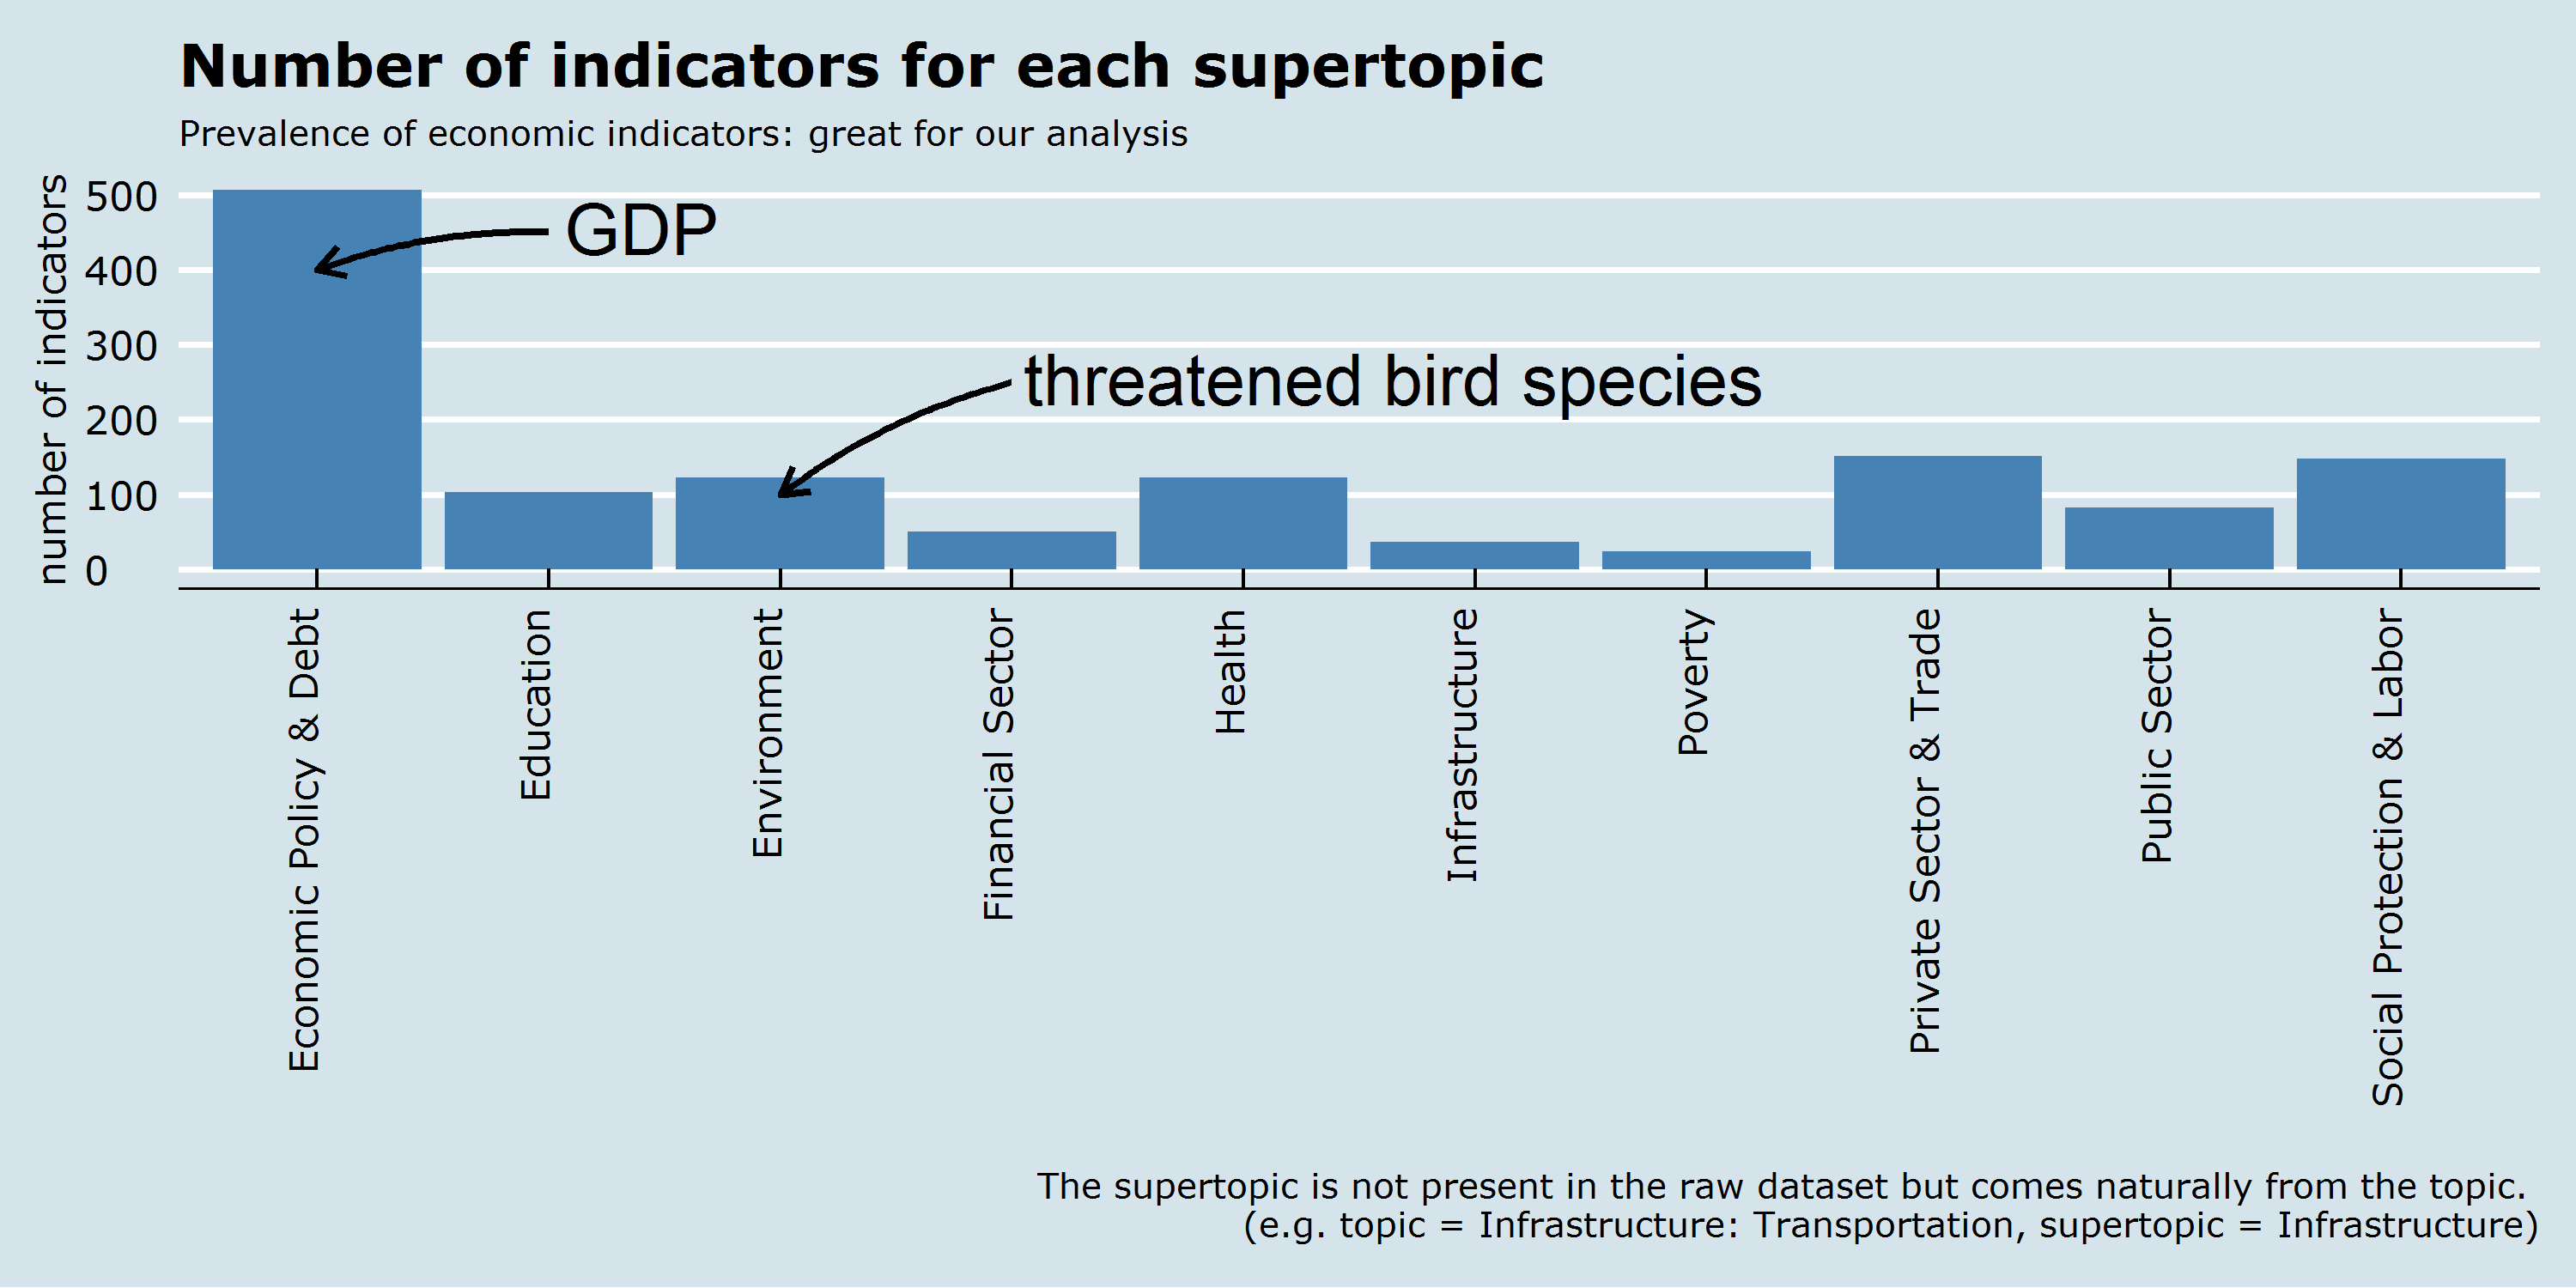
\includegraphics[width=\textwidth]{plot0004.png}
\end{figure}
\end{frame}

\begin{frame}
\begin{center}
{\Large An intermediate goal:} \\[.2cm]
Extract a full matrix with meaningful indicators to perform PCA
\end{center}
\end{frame}


\begin{frame}
\begin{figure}
\centering
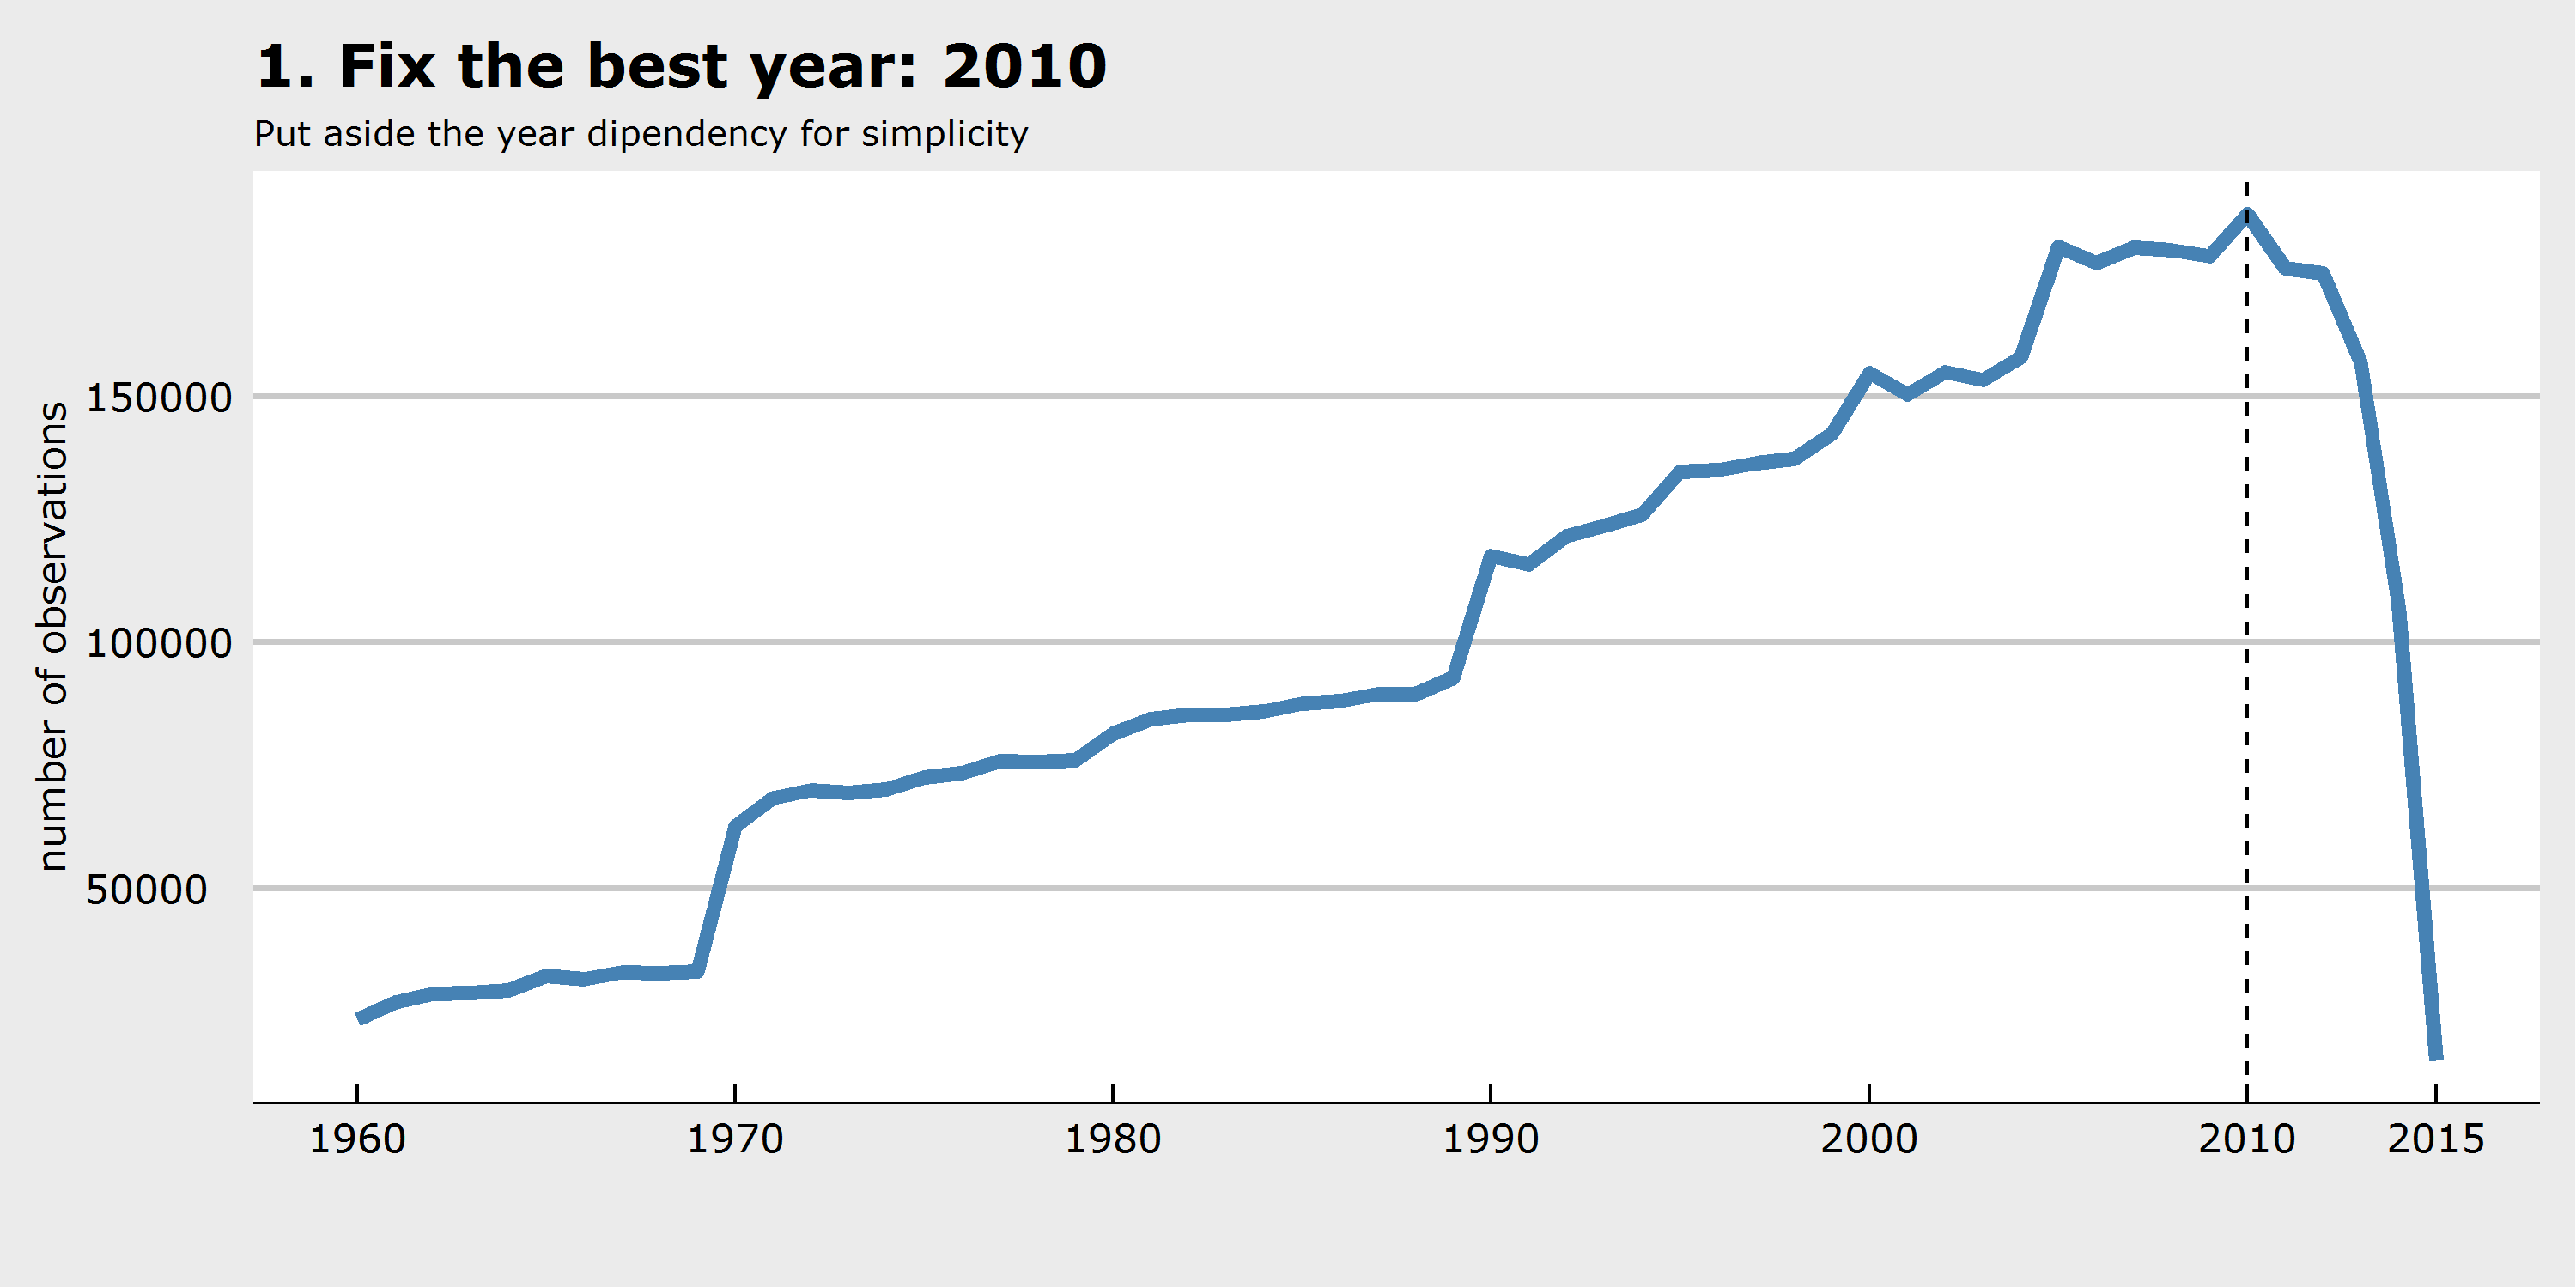
\includegraphics[width=\textwidth]{fix2010.png}
\end{figure}
\end{frame}

\begin{frame}
\begin{figure}
\centering
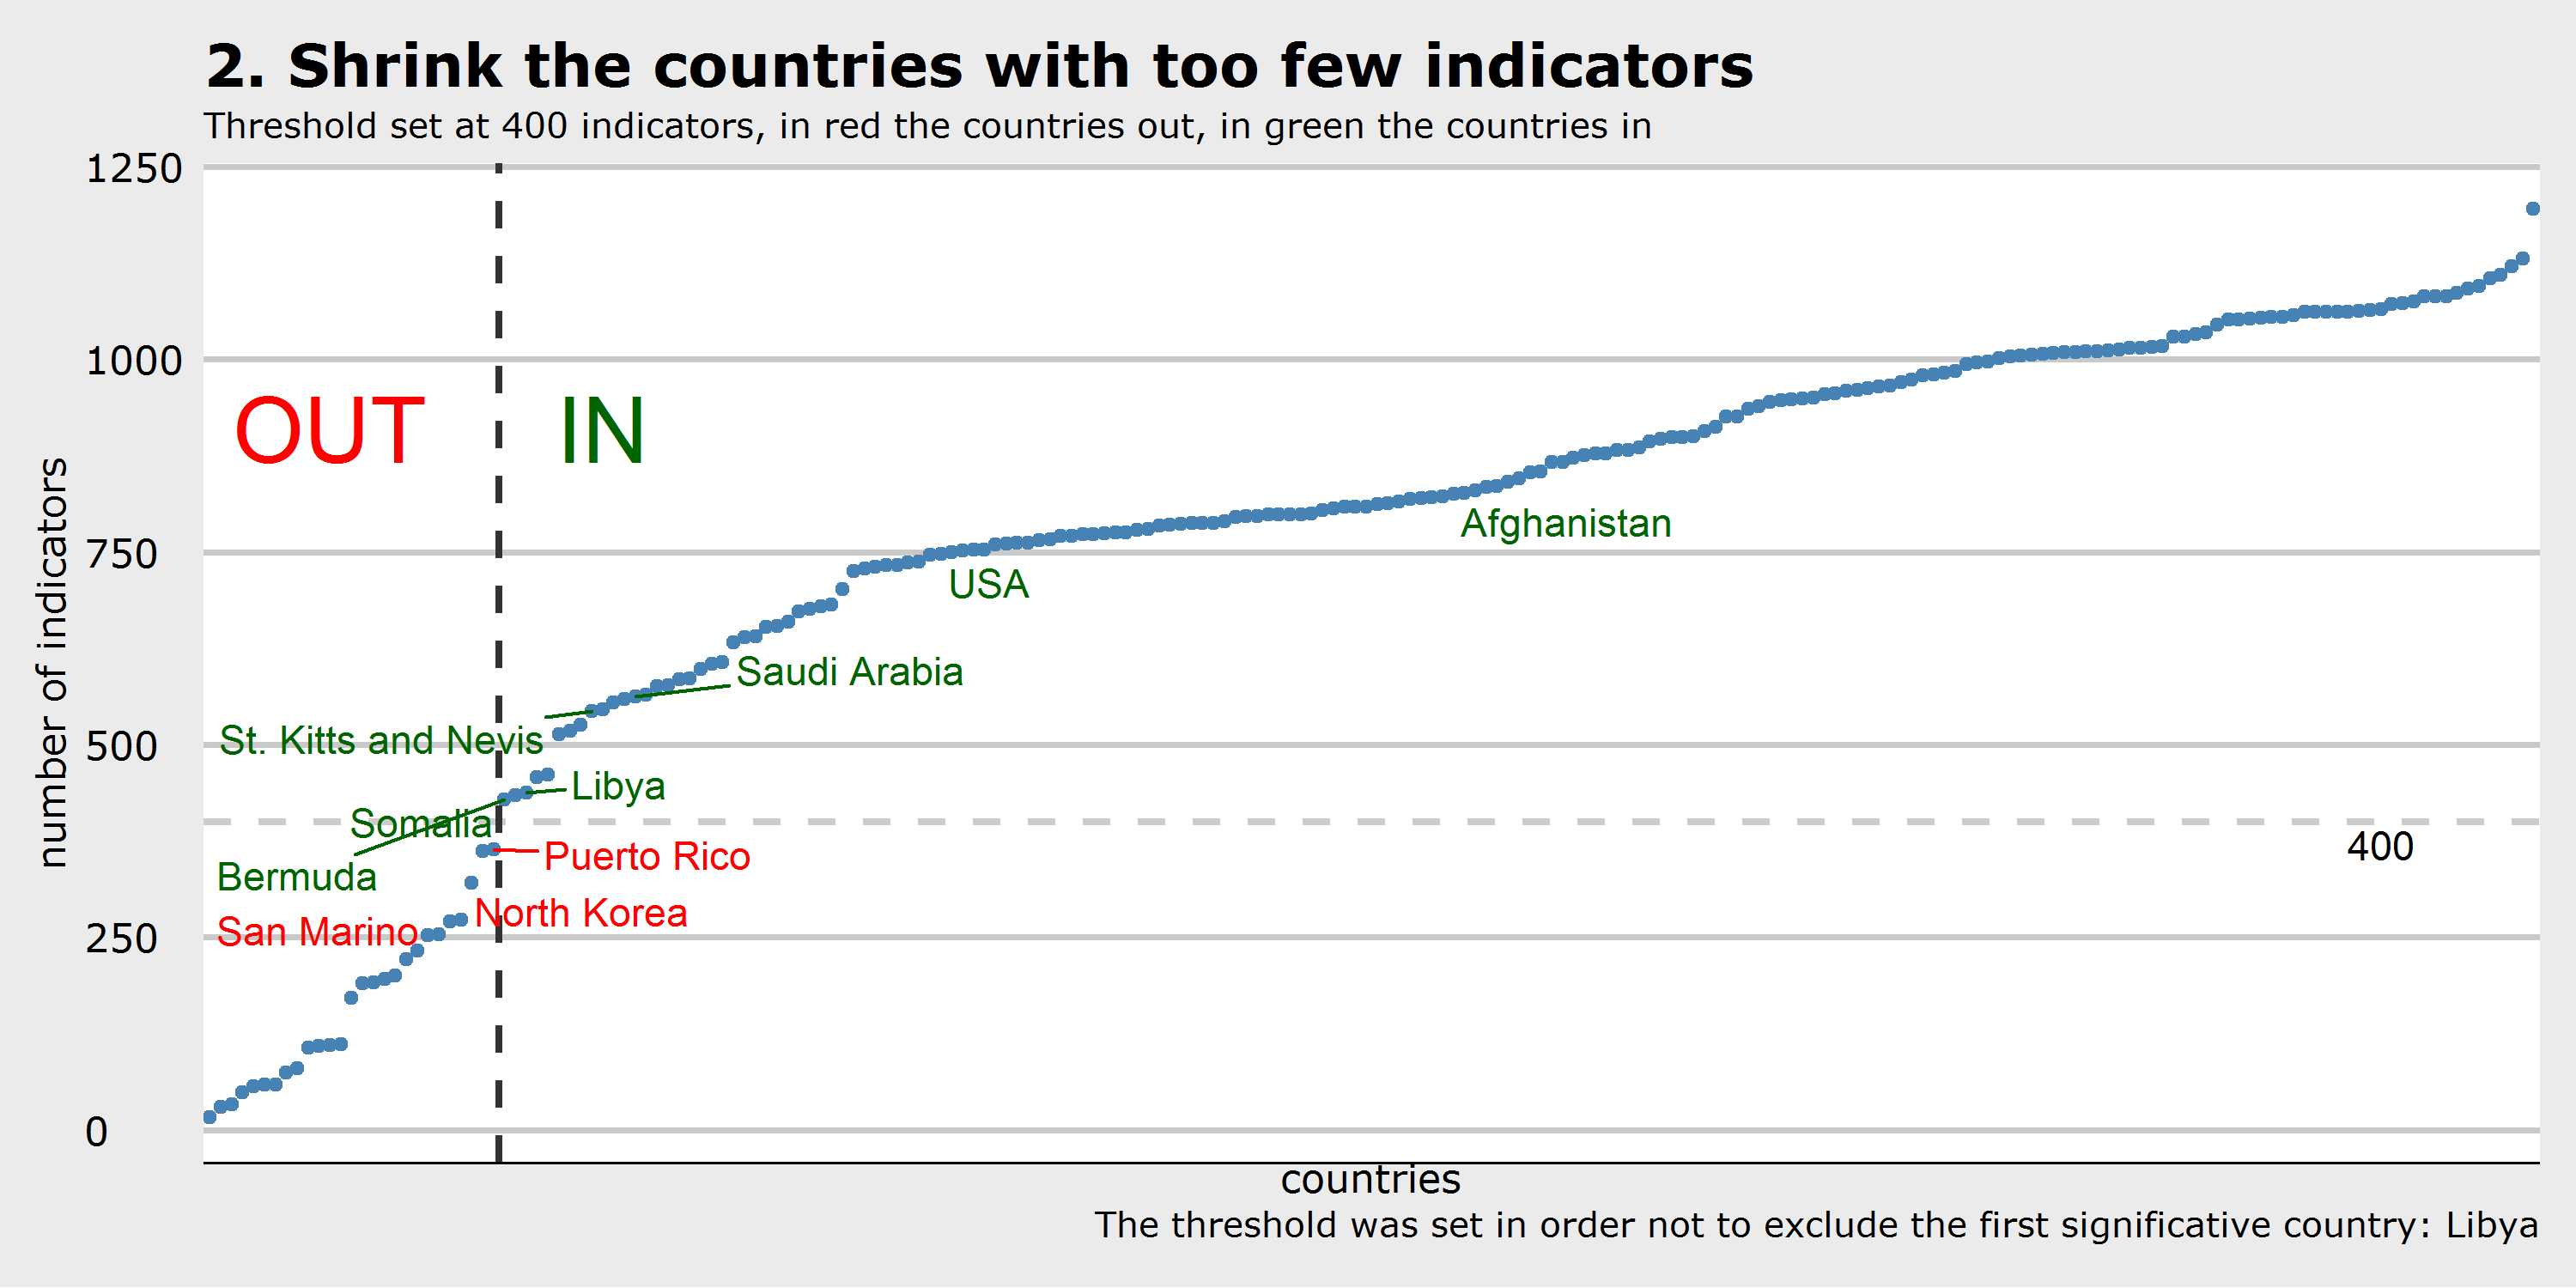
\includegraphics[width=\textwidth]{plot0005.png}
\end{figure}
\end{frame}

\begin{frame}
\begin{figure}
\centering
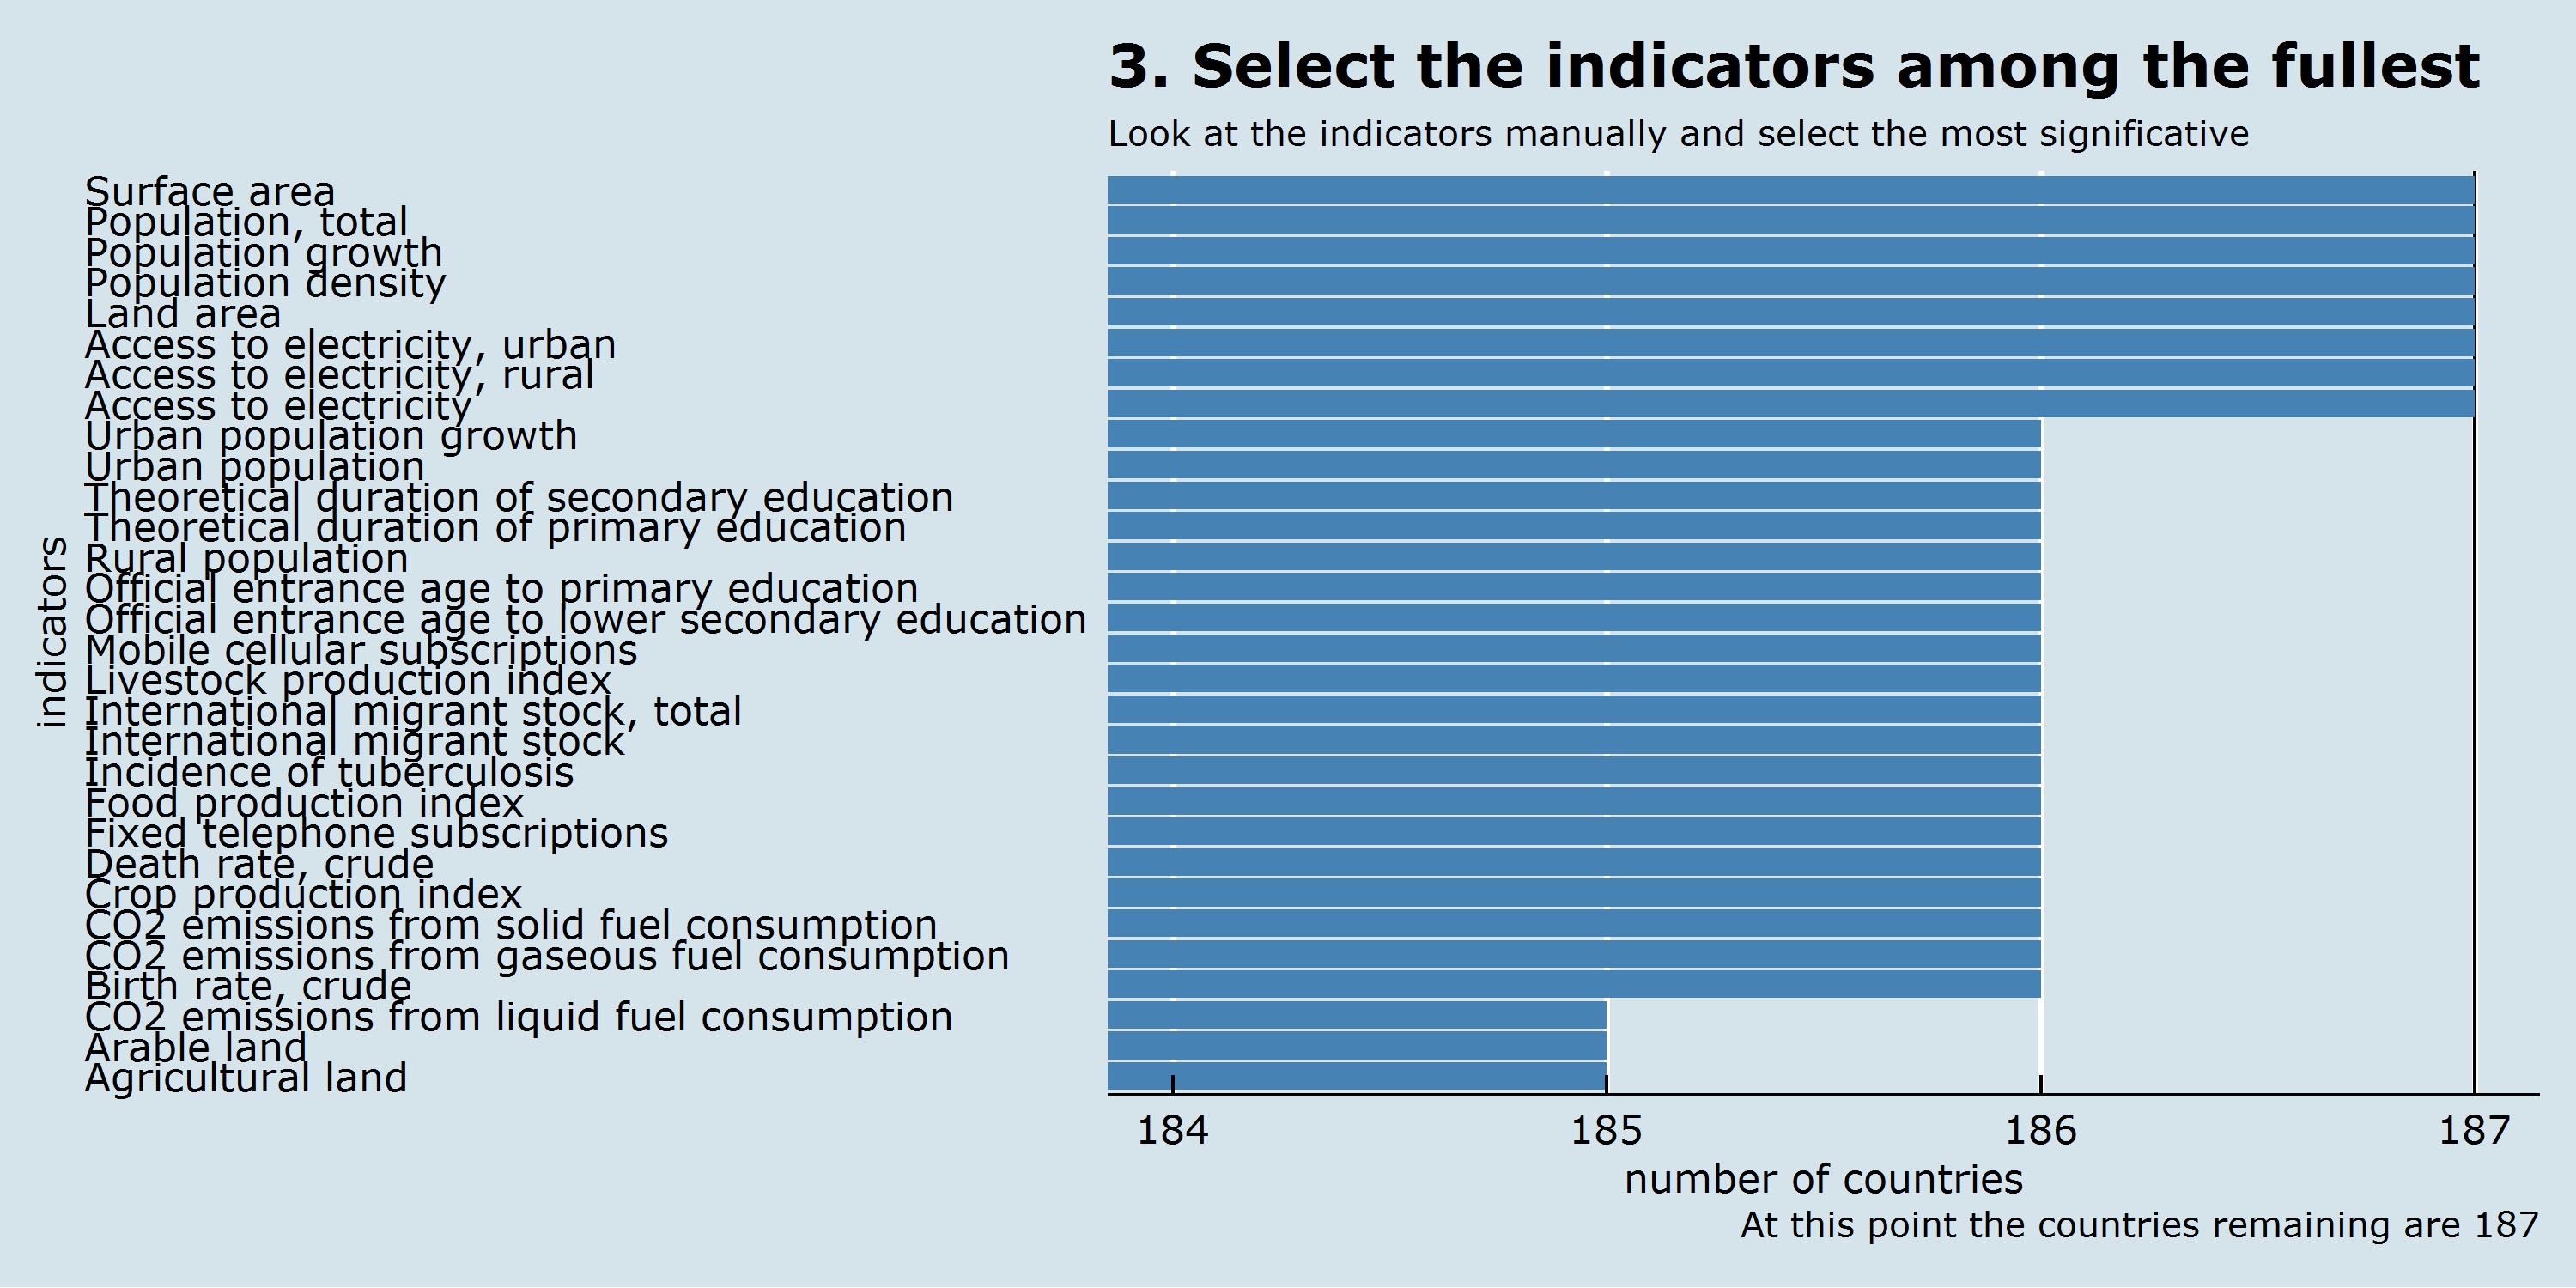
\includegraphics[width=\textwidth]{plot0006.png}
\end{figure}
\end{frame}

\begin{frame}
\begin{figure}
\centering
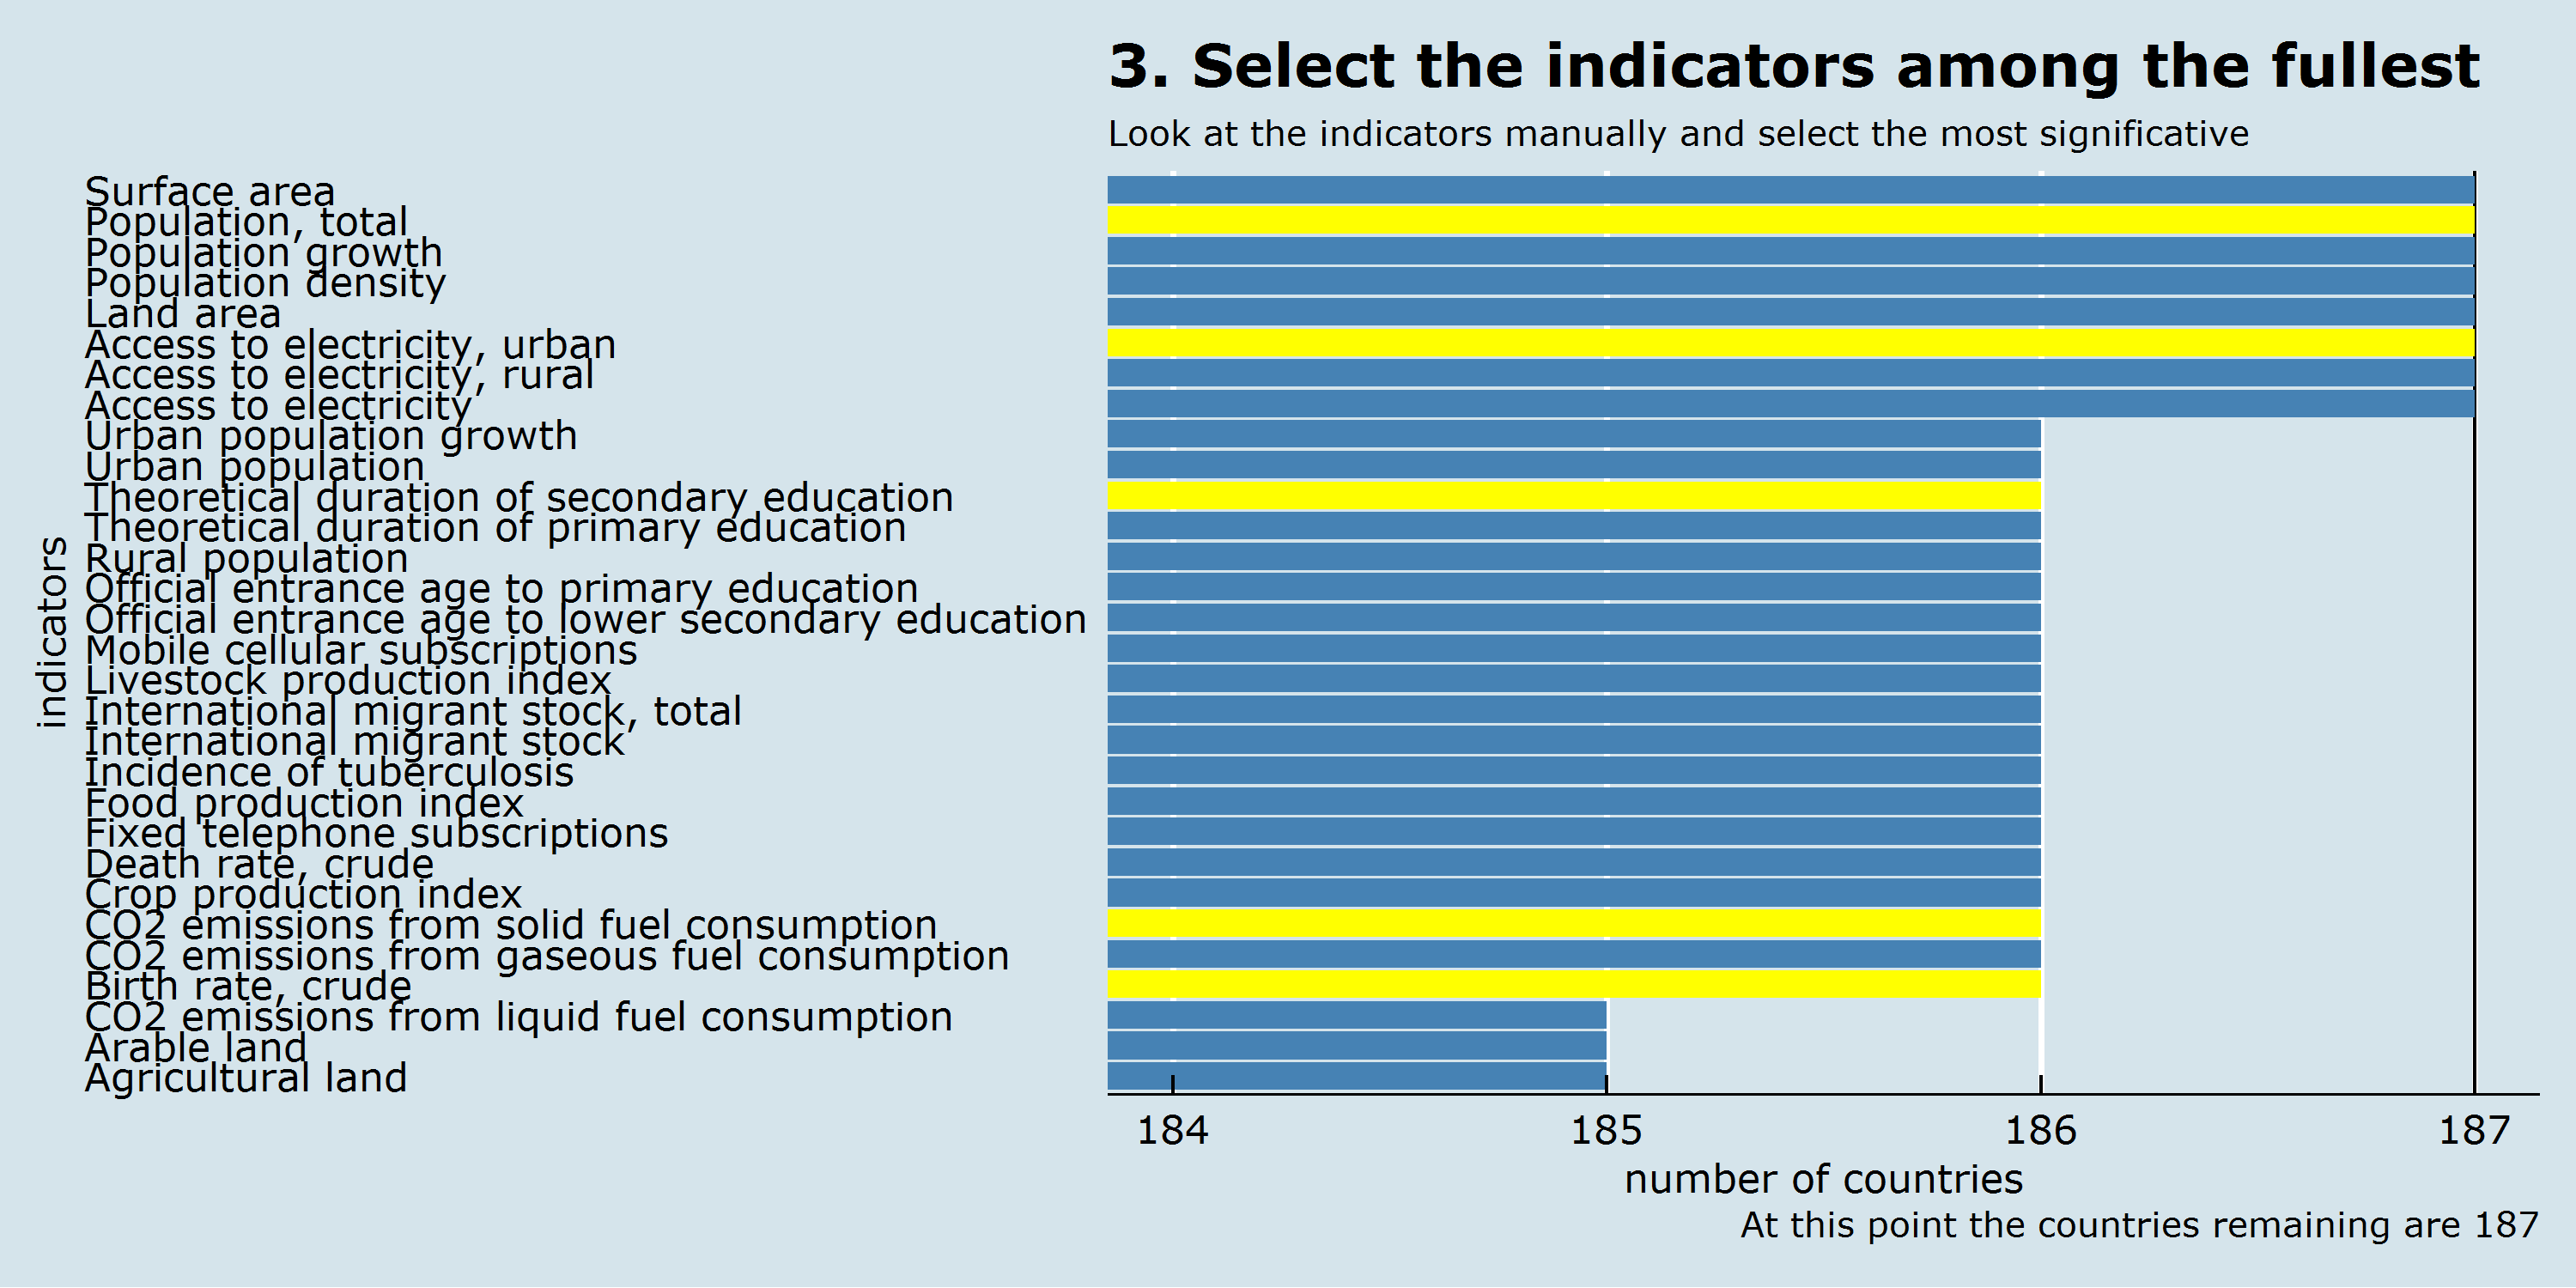
\includegraphics[width=\textwidth]{plot0007.png}
\end{figure}
\end{frame}

\begin{frame}
{Next steps:}
\begin{itemize} [<+->]
	\item[4.] Evaluate the fullness of the matrix
	\item[5.] If problematic countries or indicators are still present, consider shrinking them
	\item[6.] Fill the \textit{real} missing data (via interpolation, value at the previous year or manually from the source)
	\item[7.] Expand the shrunk matrix over years 
\end{itemize}
\end{frame}


% some examples of our indicators
\begin{frame}{Example 1}
\begin{figure}
\centering
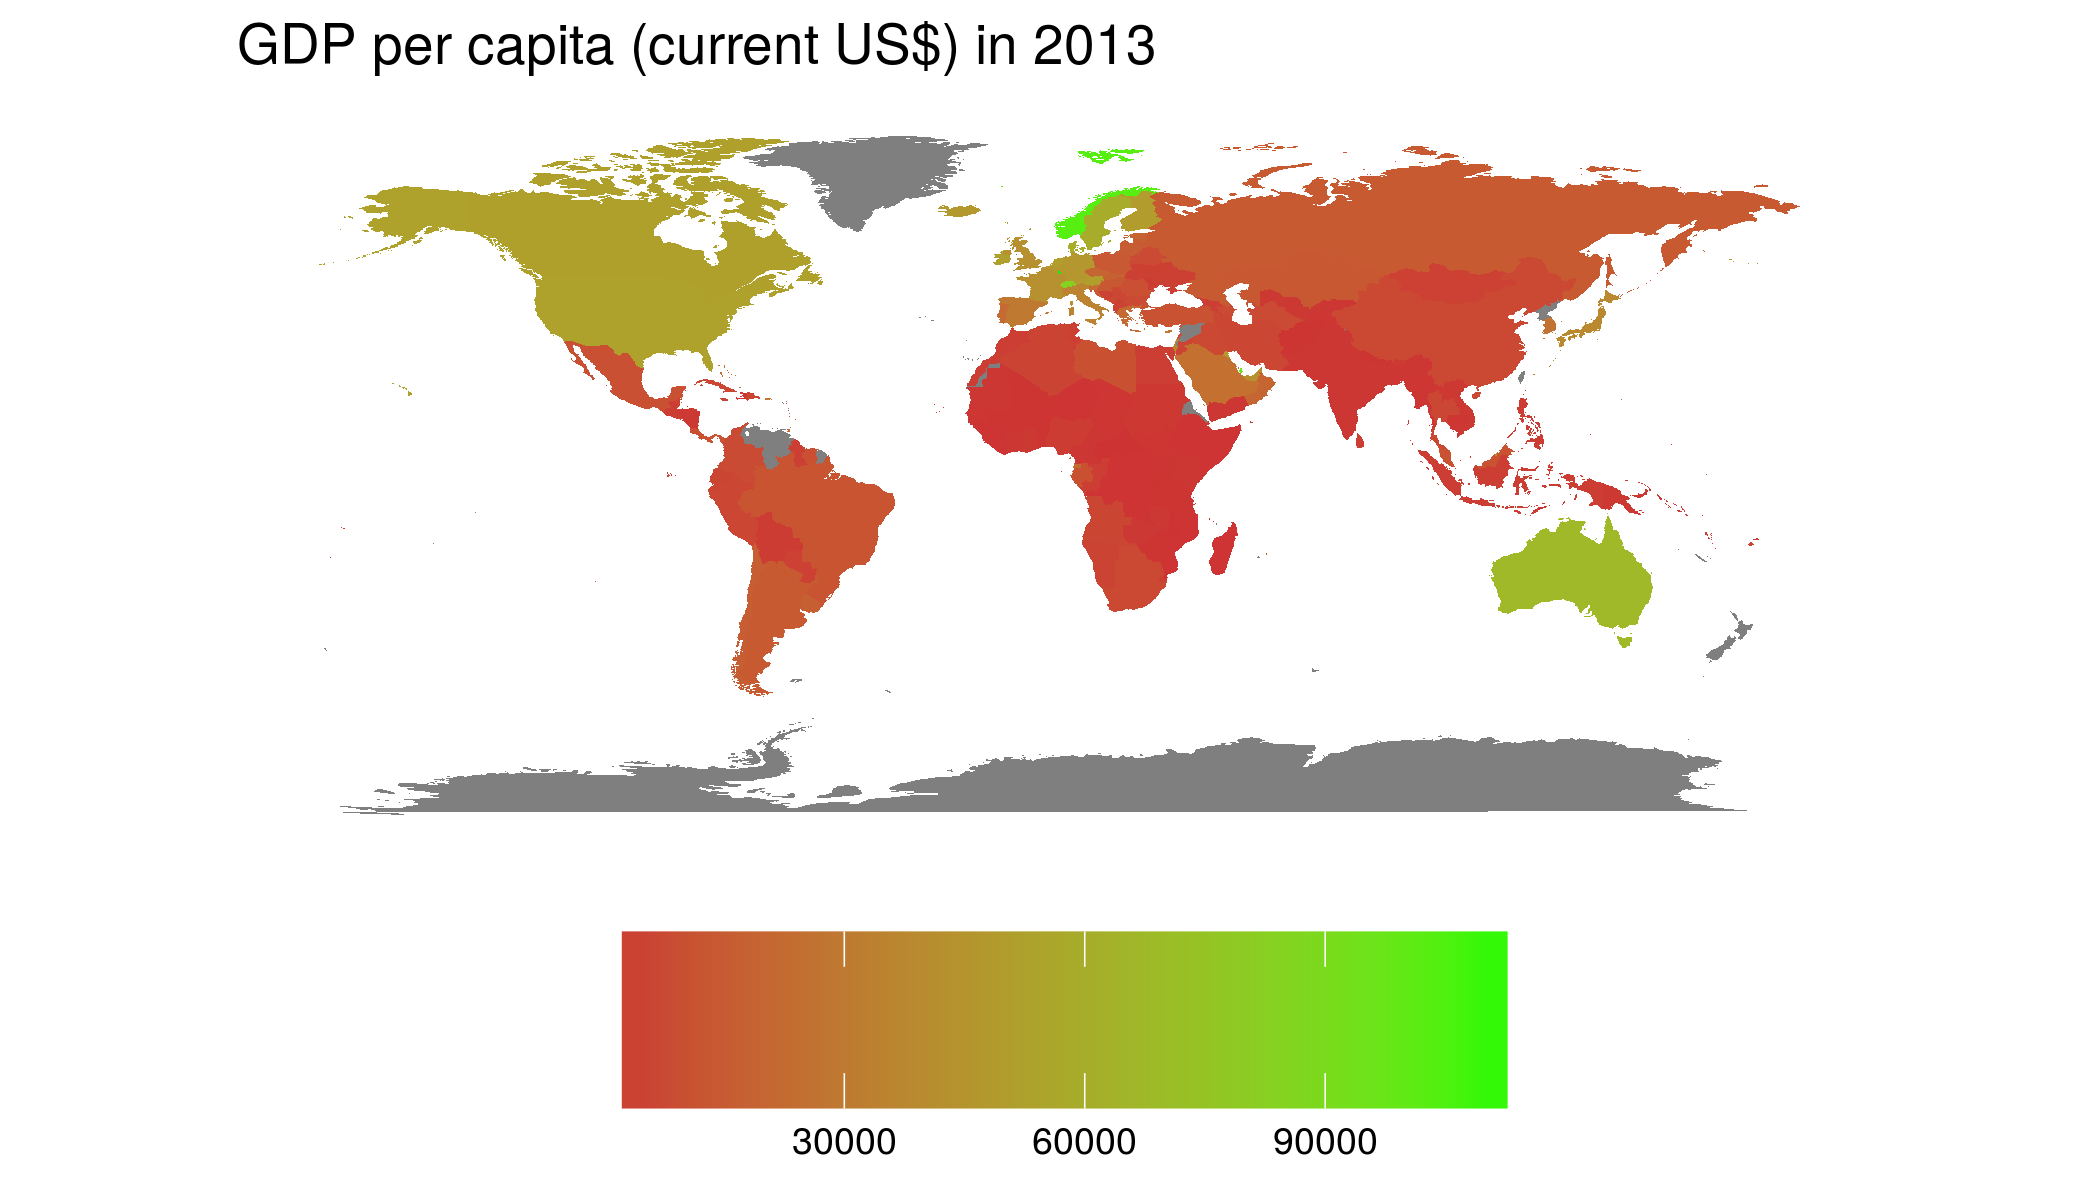
\includegraphics[width=\textwidth]{GDP.png}
\caption[GDP per capita, 2013]{GDP per capita, 2013}
\end{figure}

\end{frame}
\begin{frame}{Example 2}
\begin{figure}
\centering
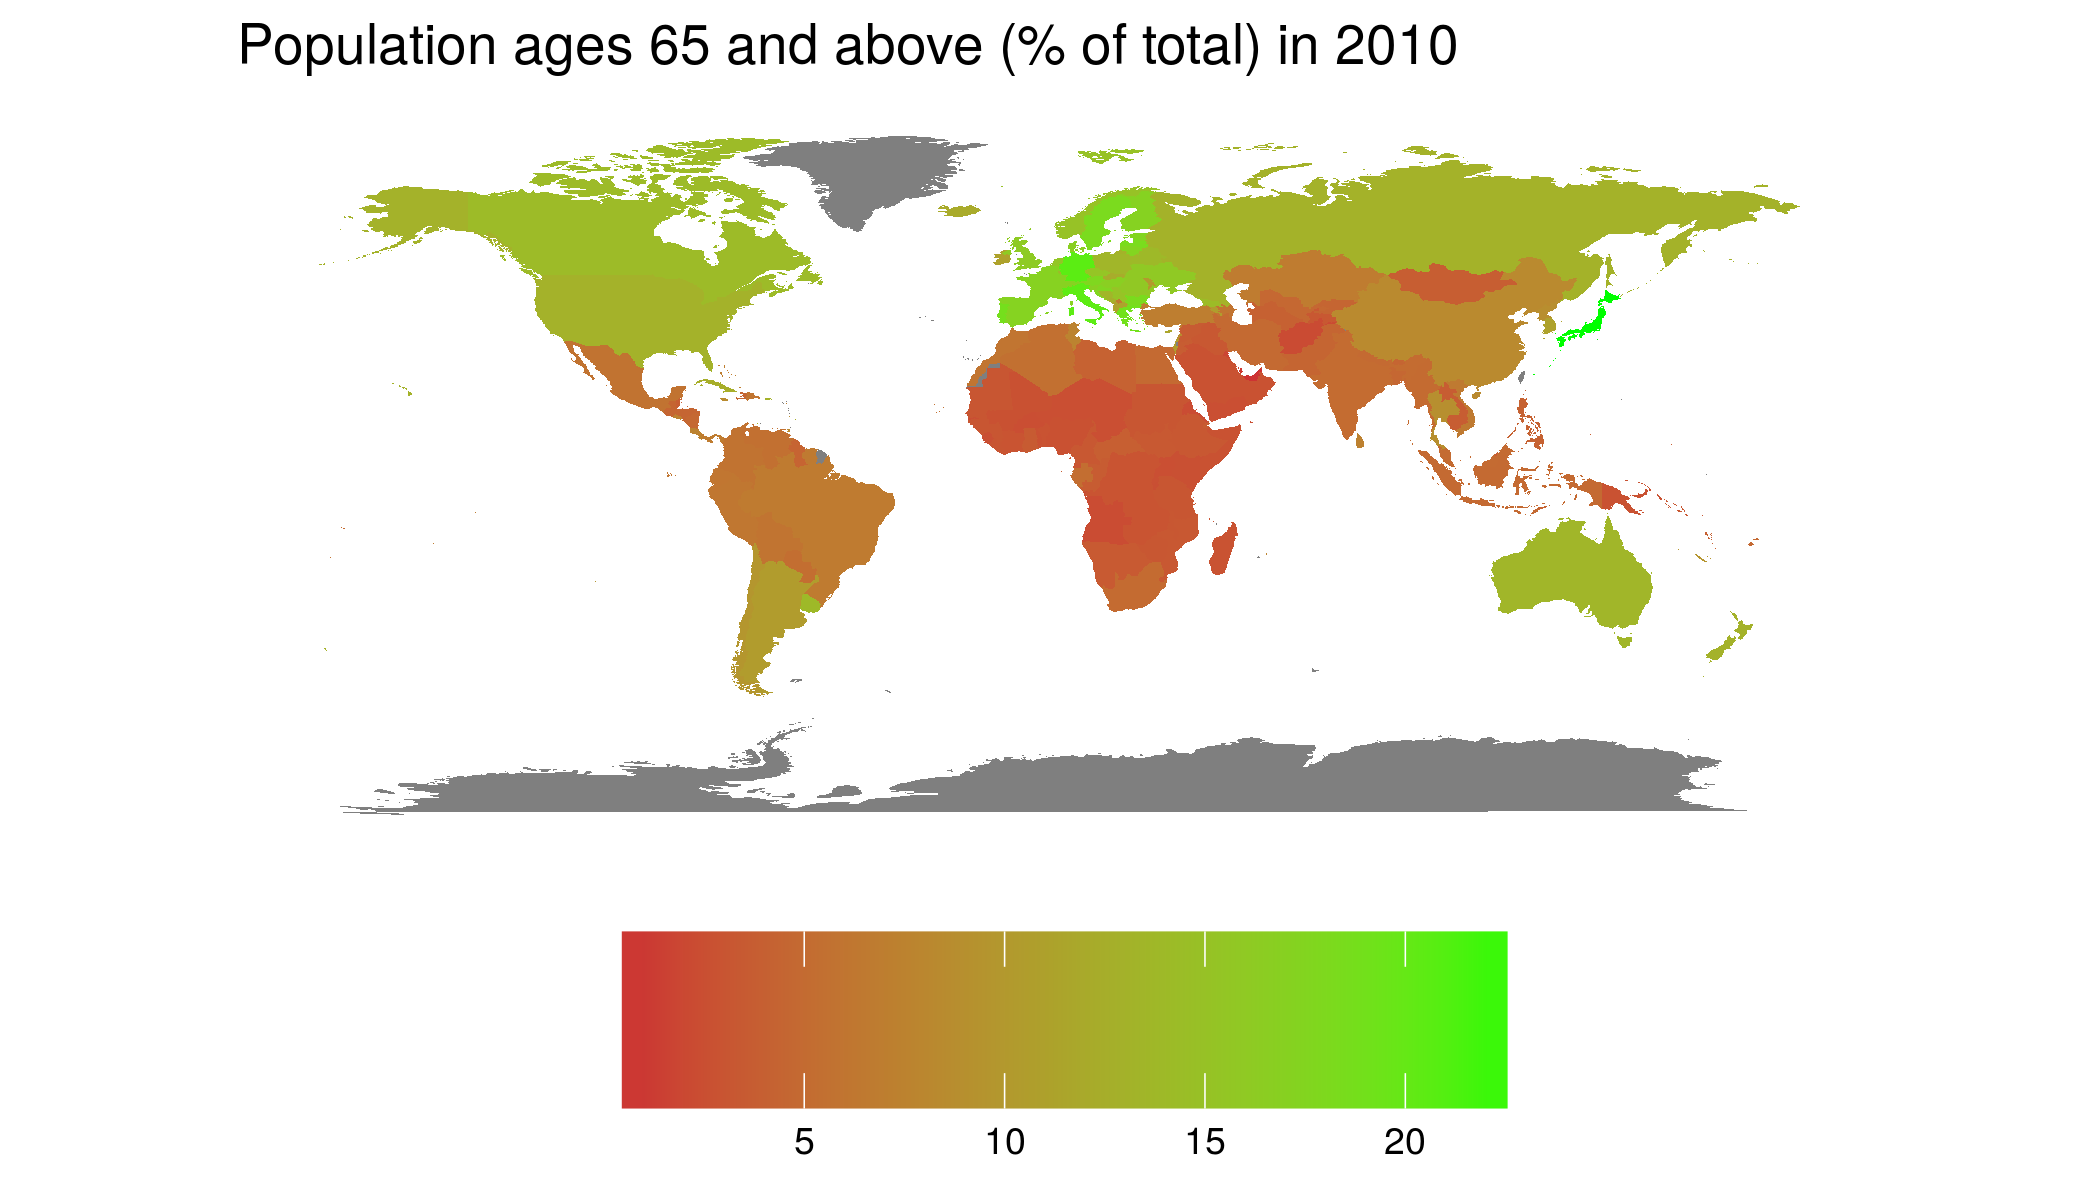
\includegraphics[width=1\textwidth]{ageing.png}
\caption[Population aged over 65]{Population aged over 65}
\end{figure}
\end{frame}

\begin{frame}{Example 3}
\begin{figure}
\centering
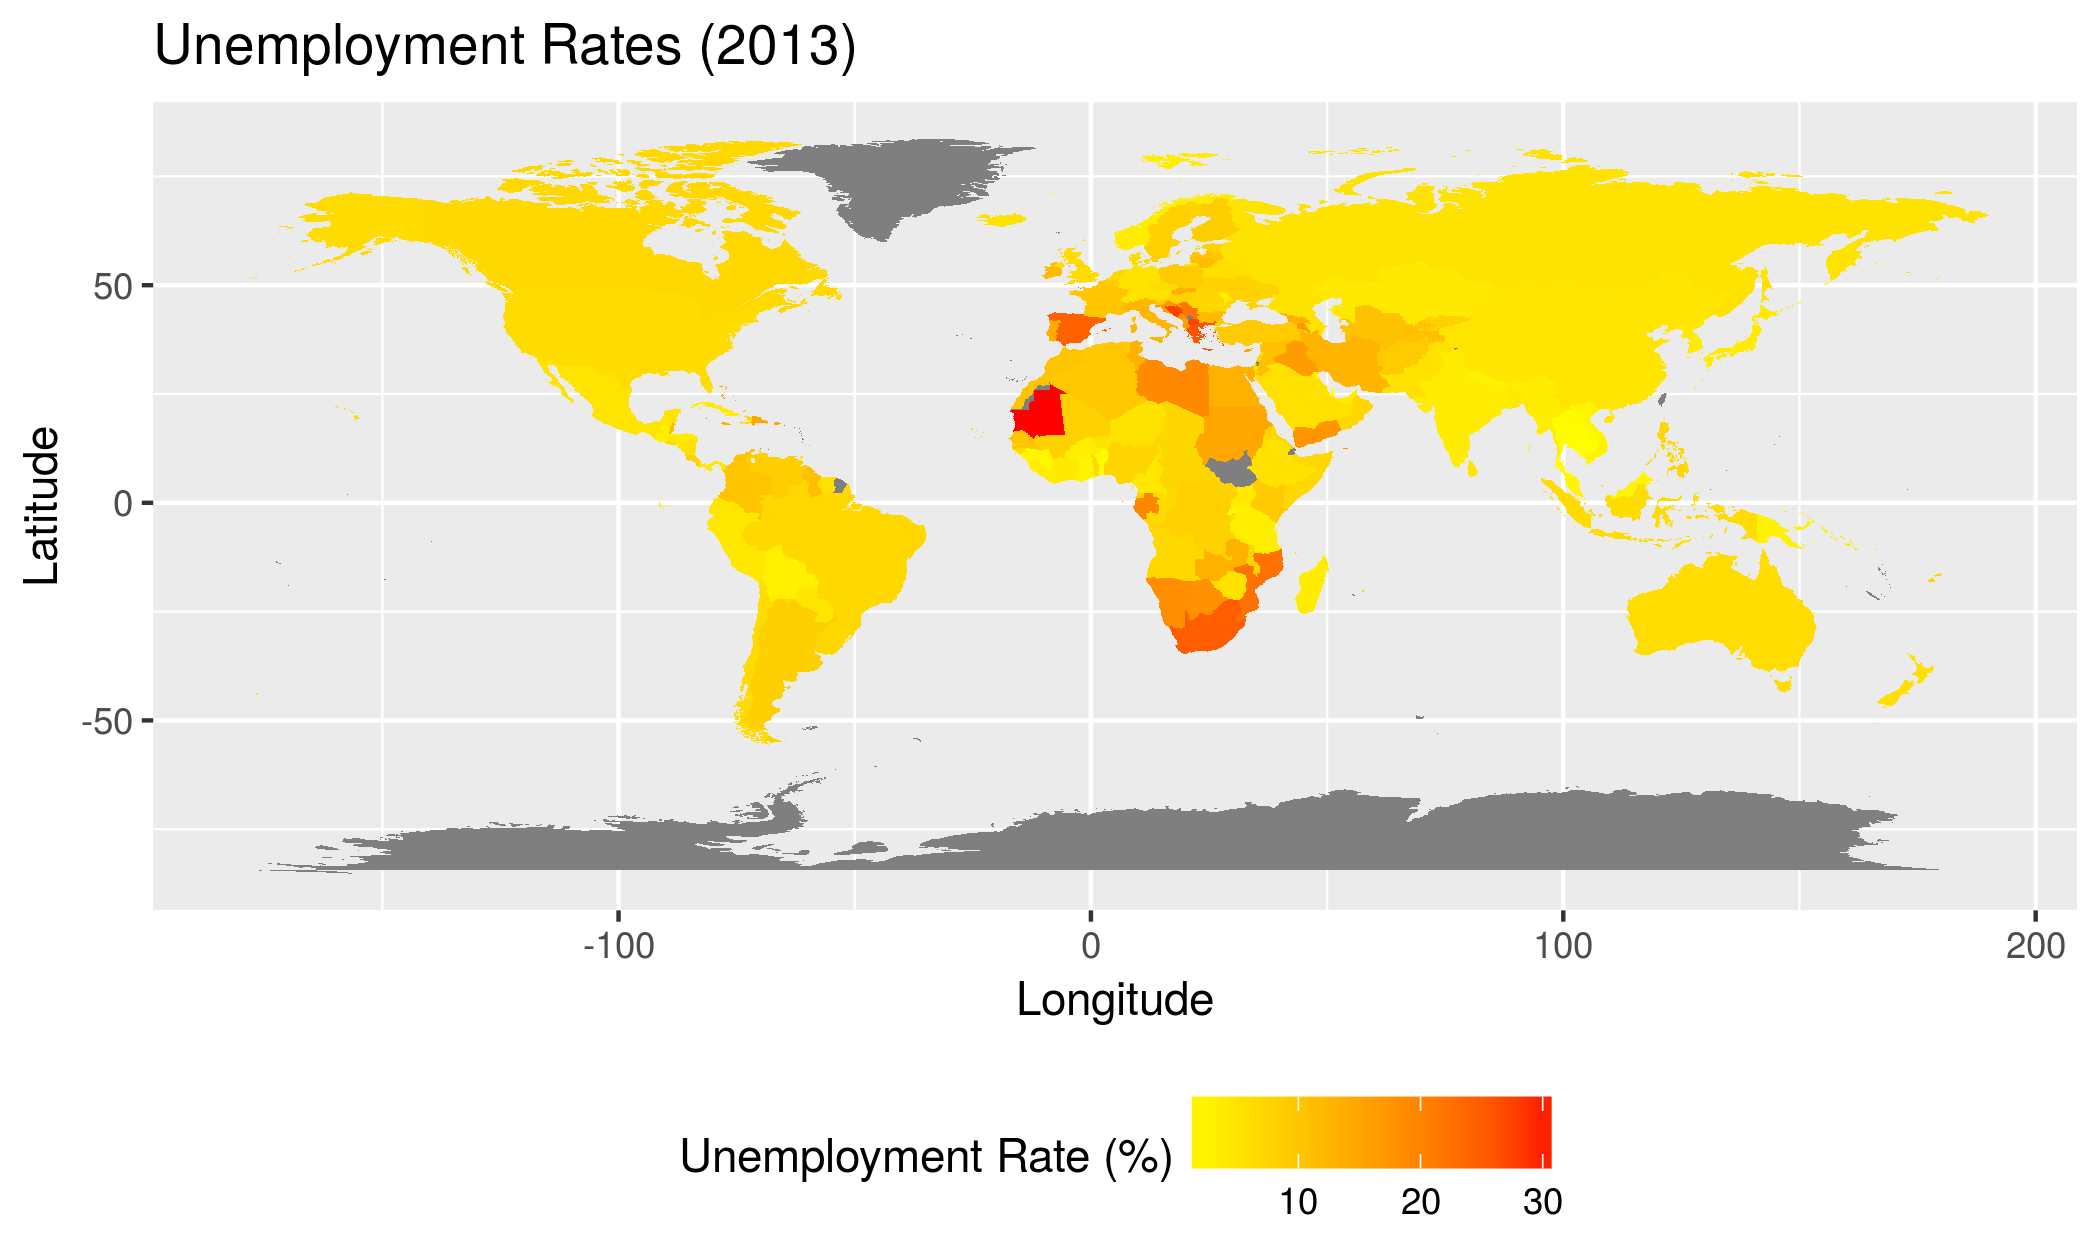
\includegraphics[width=\textwidth]{unemploy.png}
\caption[World unemployment]{World unemployment}
\end{figure}
\end{frame}

\end{document}